\documentclass[12pt,a4paper,oneside]{report}

% Pass options to url package before hyperref loads it
\PassOptionsToPackage{hyphens}{url}

% Пакети
\usepackage[utf8]{inputenc}
\usepackage[ukrainian]{babel}
\usepackage[T2A]{fontenc}
\usepackage[numbers]{natbib}  % Для налаштування бібліографії (числовий стиль)
\usepackage{geometry}
\usepackage{setspace}
\usepackage{graphicx}
\usepackage{amsmath}
\usepackage{amssymb}
\usepackage{listings}
\usepackage{xcolor}
\usepackage{hyperref}
\usepackage{tocloft}
\usepackage{titlesec}
\usepackage{fancyhdr}
\usepackage[tableposition=top]{caption}
\usepackage{subcaption}
\usepackage{longtable}
\usepackage{booktabs}
\usepackage{array}
\usepackage{multirow}
\usepackage{enumitem}
\usepackage{indentfirst}
\usepackage{microtype}

% Налаштування сторінки
\geometry{
    left=30mm,
    right=15mm,
    top=20mm,
    bottom=20mm
}

% Покращення розбиття рядків
\emergencystretch=1em
\tolerance=1000
\hyphenpenalty=500
\exhyphenpenalty=50

% Міжрядковий інтервал
\setstretch{1.5}

% ВАЖЛИВО: Відступ абзаців 1.25 см
\setlength{\parindent}{1.25cm}

% ВАЖЛИВО: Налаштування списків itemize/enumerate з інтервалом 1.5
\setlist{
    itemsep=0pt,
    parsep=0pt,
    topsep=0pt,
    partopsep=0pt
}

% Налаштування шрифтів для заголовків
\titleformat{\chapter}[hang]
    {\normalfont\bfseries\centering\fontsize{14pt}{16.8pt}\selectfont}
    {\MakeUppercase{\chaptertitlename\ \thechapter.}}
    {0.5em}
    {\MakeUppercase}
\titlespacing*{\chapter}{0pt}{0pt}{2\baselineskip}

\titleformat{\section}
    {\normalfont\bfseries\fontsize{12pt}{14.4pt}\selectfont}
    {\thesection}
    {1em}
    {}
\titlespacing*{\section}{0pt}{\baselineskip}{0pt}

\titleformat{\subsection}
    {\normalfont\bfseries\fontsize{12pt}{14.4pt}\selectfont}
    {\thesubsection}
    {1em}
    {}
\titlespacing*{\subsection}{0pt}{\baselineskip}{0pt}

% Налаштування колонтитулів
\pagestyle{fancy}
\fancyhf{}
\fancyfoot[C]{\thepage}
\renewcommand{\headrulewidth}{0pt}

% Налаштування змісту
\renewcommand{\cftchapfont}{\normalfont\bfseries}
\renewcommand{\cftsecfont}{\normalfont}
\renewcommand{\cftsubsecfont}{\normalfont}

% Налаштування підписів
\captionsetup{
    labelsep=space,
    justification=centering,
    singlelinecheck=false,
    font={normalsize,normalfont},
    labelfont={normalsize,normalfont}
}

\captionsetup[table]{
    position=top,
    skip=10pt,
    justification=raggedright,
    singlelinecheck=false,
    font={normalsize,normalfont},
    labelfont={normalsize,normalfont}
}

\captionsetup[figure]{
    position=bottom,
    justification=centering,
    font={normalsize,normalfont},
    labelfont={normalsize,normalfont}
}

% Налаштування listings для коду
\lstset{
    basicstyle=\ttfamily\small,
    breaklines=true,
    frame=single,
    numbers=left,
    numberstyle=\tiny,
    tabsize=4,
    showstringspaces=false
}

% Для коду в додатках
\lstdefinestyle{code}{
    basicstyle=\fontfamily{pcr}\selectfont\scriptsize,
    breaklines=true,
    frame=none,
    numbers=left,
    numberstyle=\tiny,
    tabsize=4
}

% Гіперпосилання
\hypersetup{
    colorlinks=true,
    linkcolor=black,
    citecolor=black,
    urlcolor=blue
}

% Метадані
\title{IndustryFlow: Платформа IoT MLOps для моніторингу промислових сенсорів}
\author{Костянтин Романчук}
\date{Листопад 2025}

\begin{document}

% Титульна сторінка (без нумерації)
\pagenumbering{gobble}
\thispagestyle{empty}

\begin{center}

\vspace*{1cm}

% Логотип Woolf вгорі

\includegraphics[width=0.25\textwidth]{figures/woolf.png}

\vspace{2cm}

% Назва роботи (лапки та звичайний шрифт)
% Пояснювальна записка
{\fontsize{18pt}{21.6pt}\selectfont\bfseries
``Розробка горизонтально масштабованої multi-tenant платформи для моніторингу промислових IoT-систем у реальному часі з ML-детекцією аномалій''
}

\vspace{1cm}

% Автор
{\fontsize{12pt}{14.4pt}\selectfont
Автор: Костянтин Романчук
}

\vspace{2cm}

{\fontsize{12pt}{14.4pt}\selectfont Пояснювальна записка до дипломної роботи, подана до Neoversity на здобуття ступеня 
Master of Science in Computer Science
}


\vspace{1cm}

% Дата
{\fontsize{12pt}{14.4pt}\selectfont
Листопад, 2025
}

\vspace{2cm}

% Логотип Neoversity

\includegraphics[width=0.5\textwidth]{figures/neovercity.png}

\vspace{3cm}

% Інформація про студента
\begin{flushleft}
{\fontsize{12pt}{13.2pt}\selectfont
Студентський номер: 1045351359 \\[0.3em]
Науковий керівник: PhD. Тетяна Філімонова \\[0.3em]
}\end{flushleft}

\end{center}

\vspace{1cm}

\noindent
{\fontsize{12pt}{12pt}\selectfont
© Пояснювальна записка до дипломної роботи Костянтина Романчука затверджена й відповідає вимогам щодо якості та оформлення для електронної публікації.
}
\clearpage

% Початок арабської нумерації з сторінки 1
\pagenumbering{arabic}
\setcounter{page}{1}

% Сертифікація
%\thispagestyle{empty}

\begin{center}
{\fontsize{14pt}{16.8pt}\selectfont\bfseries
СЕРТИФІКАЦІЯ ПОЯСНЮВАЛЬНОЇ ЗАПИСКИ ДО ДИПЛОМНОЇ РОБОТИ
}
\end{center}

\vspace{2cm}

Я підтверджую, що я аналізував цей проєкт і, на мою думку, він відповідає належним стандартам академічної презентації. Я вважаю, що він задовільно відповідає критеріям як з точки зору якості, так і з точки зору обсягу, щоб слугувати пояснювальною запискою до дипломної роботи для здобуття наукового ступеня Master of Science in Computer Science.

\vspace{1cm}

Ця пояснювальна записка до дипломної роботи була подана до Neoversity та вважається достатньою для виконання передумов для здобуття наукового ступеня Master of Science in Computer Science.

\vspace{4cm}

\noindent
\rule{0.4\textwidth}{0.4pt}

\noindent
PhD. Тетяна Філімонова


\clearpage

% Декларація
%\thispagestyle{empty}

\begin{center}
{\fontsize{14pt}{16.8pt}\selectfont\bfseries
ДЕКЛАРАЦІЯ АКАДЕМІЧНОЇ ДОБРОЧЕСНОСТІ
}
\end{center}

\vspace{2cm}

Я підтверджую, що ця пояснювальна записка до дипломної роботи, подана на виконання вимог для здобуття ступеня Master of Science in Computer Science, виконана мною з [дата початку] до [дата закінчення], є результатом моєї особистої роботи. Будь-який внесок із зовнішніх джерел або окремих осіб, зокрема використання інструментів штучного інтелекту, належним чином підтверджено шляхом цитування. Крім того, я підтверджую, що цей матеріал не був раніше поданий, повністю або частково, для здобуття наукового ступеня в цій або будь-якій іншій установі. Роблячи цю заяву, я визнаю й розумію, що будь-яке порушення цього положення є академічним проступком й може призвести до відрахування з програми та/або позбавлення права на здобуття наукового ступеня.

\vspace{1cm}

\vspace{4cm}

\noindent
Костянтин Романчук: \rule{0.3\textwidth}{0.4pt}\hspace{1cm} [Дата]

\clearpage

% Анотація (українською)
\chapter*{АНОТАЦІЯ}
\addcontentsline{toc}{chapter}{АНОТАЦІЯ}

Ця робота присвячена розробці платформи IoT MLOps для моніторингу промислових сенсорів у реальному часі з виявленням аномалій на основі машинного навчання.

Актуальність дослідження обумовлена потребою промислових підприємств у доступних рішеннях для моніторингу обладнання. Існуючі корпоративні платформи мають високу вартість та складність впровадження, тоді як рішення з відкритим кодом потребують значних зусиль для інтеграції компонентів.

Метою роботи є створення багатокористувацької платформи, що поєднує потокову обробку даних, машинне навчання для детекції аномалій та MLOps практики на базі технологій з відкритим кодом.

Методологія включає аналітичний метод для вивчення існуючих платформ, методи машинного навчання (Isolation Forest, Random Forest, XGBoost) для детекції аномалій, експериментальний метод для тестування продуктивності та порівняльний аналіз алгоритмів.

Основні результати: розроблено мікросервісну архітектуру на базі Docker; забезпечено потокову обробку даних з низькою затримкою через Apache Kafka та Spark; реалізовано схема-на-тенанта ізоляцію зі стисненням TimescaleDB; досягнуто високу якість детекції аномалій на наборі даних Tennessee Eastman Process.

Практична значущість полягає у створенні готового рішення для промислових підприємств, що забезпечує раннє виявлення несправностей обладнання та зниження витрат на незаплановане обслуговування.

\vspace{1cm}

\noindent
\textbf{Ключові слова:} IoT, MLOps, виявлення аномалій, промисловий моніторинг, TimescaleDB, Apache Kafka, Apache Spark, машинне навчання, мікросервісна архітектура

\clearpage

% Анотація (англійською)
\chapter*{ABSTRACT}
\addcontentsline{toc}{chapter}{ABSTRACT}

This paper presents a methodology for developing an IoT MLOps platform for real-time industrial sensor monitoring with machine learning-based anomaly detection. The approach combines stream data processing through Apache Kafka and Apache Spark Structured Streaming with a multi-tenant schema-per-tenant architecture in TimescaleDB. The system employs anomaly detection algorithms with MLflow infrastructure for experiment tracking and model versioning. Experimental results demonstrate the effectiveness of stream processing, data compression, and anomaly detection quality on a benchmark dataset. This work provides a production-ready solution for industrial enterprises enabling early detection of equipment failures using open-source technologies.

Keywords: IoT, MLOps, anomaly detection, industrial monitoring, TimescaleDB, Apache Kafka, Apache Spark, machine learning, microservices architecture.

\clearpage

% Подяки (за бажанням)
% \input{sections/05_acknowledgments}
% \clearpage

% Зміст
\tableofcontents
\clearpage

% Список таблиць
\listoftables
\clearpage

% Список рисунків
\listoffigures
\clearpage

% Список скорочень
\chapter*{СПИСОК СКОРОЧЕНЬ}
\addcontentsline{toc}{chapter}{СПИСОК СКОРОЧЕНЬ}


\begin{longtable}{|p{3cm}|p{10cm}|}
\hline
\textbf{Скорочення} & \textbf{Повна назва} \\
\hline
\endfirsthead

\hline
\textbf{Скорочення} & \textbf{Повна назва} \\
\hline
\endhead

\textbf{ABAC} & Attribute-Based Access Control \\
\hline
\textbf{AI} & Artificial Intelligence (Штучний інтелект) \\
\hline
\textbf{AUC} & Area Under the Curve \\
\hline
\textbf{CI/CD} & Continuous Integration/Continuous Deployment \\
\hline
\textbf{CoAP} & Constrained Application Protocol \\
\hline
\textbf{CRM} & Customer Relationship Management \\
\hline
\textbf{ERP} & Enterprise Resource Planning \\
\hline
\textbf{GAN} & Generative Adversarial Network \\
\hline
\textbf{GDPR} & General Data Protection Regulation \\
\hline
\textbf{HDFS} & Hadoop Distributed File System \\
\hline
\textbf{HIPAA} & Health Insurance Portability and Accountability Act \\
\hline
\textbf{HR} & Human Resources \\
\hline
\textbf{HTTP} & HyperText Transfer Protocol \\
\hline
\textbf{IDS} & Intrusion Detection System \\
\hline
\textbf{IIoT} & Industrial Internet of Things (Промисловий Інтернет речей) \\
\hline
\textbf{IoT} & Internet of Things (Інтернет речей) \\
\hline
\textbf{LOF} & Local Outlier Factor \\
\hline
\textbf{ML} & Machine Learning (Машинне навчання) \\
\hline
\textbf{MLOps} & Machine Learning Operations \\
\hline
\textbf{MQTT} & Message Queuing Telemetry Transport \\
\hline
\textbf{OPC UA} & Open Platform Communications Unified Architecture \\
\hline
\textbf{RBAC} & Role-Based Access Control \\
\hline
\textbf{SaaS} & Software as a Service \\
\hline
\textbf{SMOTE} & Synthetic Minority Oversampling Technique \\
\hline
\textbf{SOC} & Service Organization Control \\
\hline
\textbf{USAD} & UnSupervised Anomaly Detection \\
\hline
\end{longtable}
\clearpage

% Основний текст (нумерація продовжується)

% Розділ 1: Вступ
\chapter{ВСТУП}

\section{Контекст та актуальність}

Промислові підприємства стикаються з несподіваними поломками обладнання. Це коштує дорого і забирає час. Інтернет речей в комбінації з машинним навчанням можуть допомогти, адже вони дозволяють відстежувати обладнання в реальному часі та передбачати поломки. Традиційні системи SCADA та корпоративні платформи IoT теж виконують ці функції, але мають недоліки:

\begin{itemize}
    \item висока вартість --- рішення від SAP, Siemens, GE коштують від сотень тисяч до мільйонів доларів, малі та середні підприємства не можуть собі цього дозволити;
    \item складна інтеграція --- впровадження SCADA займає від 6 місяців до 2 років, потрібні спеціалісти для налаштування, відсутність стандартів ускладнює підключення до існуючої інфраструктури;
    \item погана масштабованість --- монолітна архітектура створює вузькі місця при збільшенні кількості сенсорів, горизонтальне масштабування потребує серйозних змін або повної заміни системи;
    \item прості сповіщення --- традиційні системи використовують фіксовані пороги для окремих параметрів, вони не бачать складні аномалії, коли проблема виникає від комбінації параметрів;
    \item ізоляція даних --- коли кілька компаній використовують спільну інфраструктуру, потрібна надійна ізоляція промислових даних, більшість традиційних систем не розраховані на багатокористувацький режим.
\end{itemize}

Ці обмеження створюють потребу в новій платформі, яка має поєднувати доступність технологій з відкритим кодом, корпоративну надійність та машинне навчання для виявлення аномалій.


\section{Проблема}

Основні проблеми промислового Інтернету речей:

\begin{itemize}
    \item високий поріг входу --- підприємствам потрібне надійне відстеження обладнання, але корпоративні рішення закриті та прив'язують до одного постачальника;
    \item технічна складність --- створити власну систему важко, потрібна експертиза в розподілених системах, обробці даних в реальному часі, машинному навчанні та безпеці, це вимагає команду спеціалістів та інвестиції в розробку;
    \item незручні інтерфейси --- інтерфейси SCADA створені інженерами для інженерів, операційним менеджерам та керівникам потрібно більше часу для освоєння цих інструментів.
\end{itemize}


\section{Мета та завдання}

Мета роботи --- створити багатокористувацьку платформу для промислового моніторингу, яка масштабується, працює в реальному часі та виявляє аномалії через машинне навчання на технологіях з відкритим кодом.

Завдання дослідження:

\begin{enumerate}
    \item спроектувати мультитенантну архітектуру з окремою схемою бази даних для кожного користувача та горизонтальним масштабуванням через партиції Kafka та воркери Spark;
    \item реалізувати обробку даних в реальному часі через Apache Kafka та Apache Spark Structured Streaming з агрегаціями за періоди (1хв, 5хв, 1год);
    \item інтегрувати виявлення аномалій через три алгоритми (Isolation Forest, Random Forest, XGBoost) з MLflow для відстеження експериментів та версій моделей;
    \item створити систему сповіщень з трьома режимами детекції (порогові, ML, комбіновані);
    \item розробити REST API на FastAPI з JWT автентифікацією та документацією OpenAPI;
    \item налаштувати моніторинг через Prometheus та Grafana;
    \item протестувати систему на продуктивність, масштабованість та якість ML моделей.
\end{enumerate}


\section{Вимоги до системи}

\subsection{Функціональні вимоги}

\begin{itemize}
    \item Ф-001 Багатокористувацька архітектура (критичний) --- кожна компанія має власну схему в PostgreSQL/TimescaleDB; дані повністю ізольовані; економія 90-95\% місця через стиснення.
    \item Ф-002 Обробка в реальному часі (критичний) --- Apache Kafka та Apache Spark обробляють дані в реальному часі; автоматичні агрегації за 1хв, 5хв, 1год; затримка не більше 5 секунд.
    \item Ф-003 Виявлення аномалій (високий) --- три алгоритми (Isolation Forest, Random Forest, XGBoost); MLOps інфраструктура (MLflow, реєстр моделей, MinIO).
    \item Ф-004 Сповіщення (високий) --- CRUD операції для правил; три режими детекції (порогові, ML, комбіновані); публікація в Kafka.
    \item Ф-005 API (критичний) --- FastAPI шлюз; JWT автентифікація (7 днів); автоматичний search\_path для ізоляції; пул з'єднань; OpenAPI документація.
    \item Ф-006 Ієрархія обладнання (високий) --- гібридна архітектура з нормалізованими таблицями (Компанія → Об'єкт → Обладнання → Сенсор) та денормалізованими вимірюваннями.
    \item Ф-007 Масштабування (середній) --- горизонтальне масштабування через партиції Kafka та воркери Spark без змін коду.
\end{itemize}

\subsection{Нефункціональні вимоги}

\begin{itemize}
    \item НФ-001 Продуктивність (високий) --- асинхронне програмування FastAPI; пул з'єднань; кеш Redis (60с); мікропакетна обробка Spark; неперервні агрегати TimescaleDB.
    \item НФ-002 Безпека (критичний) --- JWT (HS256, 7 днів); Bcrypt (складність 12); ізоляція search\_path; параметризовані SQL; CORS; аудит.
    \item НФ-003 Надійність (критичний) --- доступність 99.99\%; реплікація Kafka $\geq$ 2; контрольні точки Spark; резервні копії; автовідновлення; політики перезапуску Docker.
    \item НФ-004 Зберігання (високий) --- гіпертаблиці з щоденними фрагментами; стиснення після 7 днів (90-95\%); падіння продуктивності запитів $\leq$ 20\%.
    \item НФ-005 Моніторинг (високий) --- Prometheus метрики; Grafana панелі; правила сповіщень; збереження 30 днів.
    \item НФ-006 Сумісність (середній) --- RESTful API з OpenAPI; JSON; Docker контейнери; S3-сумісний MinIO; стандартний протокол Kafka.
\end{itemize}


\section{Практична цінність}

Промислові підприємства отримують готове рішення для моніторингу обладнання на технологіях з відкритим кодом:

\begin{itemize}
    \item менше незапланованих простоїв через раннє виявлення проблем;
    \item оптимізація виробництва на основі даних;
    \item обслуговування до поломки через машинне навчання.
\end{itemize}

Інтегратори IoT можуть використовувати платформу для клієнтів без необхідності будувати все з нуля. Дослідники отримують платформу з відкритим кодом для експериментів з машинним навчанням на промислових даних з готовою інфраструктурою MLOps.

Технічні особливості платформи:

\begin{itemize}
    \item схема-на-користувача для TimescaleDB дозволяє стиснення (90-95\% економії) на відміну від захисту на рівні рядків;
    \item гібридна архітектура з нормалізованими метаданими та денормалізованими вимірюваннями забезпечує баланс між гнучкістю та швидкістю запитів;
    \item виявлення на рівні обладнання зберігає багатовимірність ознак, на відміну від аналізу кожного сенсора окремо;
    \item гібридні сповіщення поєднують пороги та моделі машинного навчання в одному механізмі.
\end{itemize}


\section{Структура роботи}

Робота складається з п'яти розділів:

\begin{itemize}
    \item Розділ 1 (Вступ) описує актуальність проблеми, мету та завдання дослідження, вимоги до системи;
    \item Розділ 2 (Огляд літератури) аналізує існуючі IoT платформи та обґрунтовує вибір технологій;
    \item Розділ 3 (Методологія) описує підхід до розробки, вибір технологій, архітектуру системи та стратегії тестування;
    \item Розділ 4 (Результати та обговорення) представляє результати тестування продуктивності, оцінку ML моделей та порівняння з існуючими рішеннями;
    \item Розділ 5 (Висновки) підсумовує досягнення цілей та окреслює напрямки подальшого розвитку.
\end{itemize}


\section{Обмеження}

Обмеження обсягу проєкту:

\begin{itemize}
    \item фокус на серверній частині та API, інтерфейс має базову функціональність;
    \item моделі машинного навчання: Isolation Forest, Random Forest, XGBoost --- глибоке навчання (LSTM, Autoencoder) залишено на майбутнє;
    \item тестування на одному сервері --- розгортання Kubernetes в перспективі.
\end{itemize}



% Розділ 2: Огляд літератури
\chapter{ОГЛЯД ЛІТЕРАТУРИ}

Промислові підприємства ставлять IoT для моніторингу обладнання та оптимізації виробництва. Однак виникає проблема: тисячі сенсорів генерують великі обсяги даних, які треба обробляти в реальному часі, знаходити аномалії та приймати рішення автоматично.

У статті \cite{alabadi2022industrial} автори описують Індустрію 4.0 --- це зміни у виробництві, торгівлі, транспорті та нафтовій галузі через Промисловий IoT. Це підвищує продуктивність і дає змогу обладнанню з різних локацій працювати разом.

Автори описали стан Індустрії 4.0 та IIoT з обмеженнями та досягненнями. Розглянули архітектуру, концепції та приклади застосування IIoT. Окрема увага була приділена технологіям, що підтримують Індустрію 4.0. Автори виділяють три напрями розвитку IIoT: глибинне навчання, периферійні обчислення та великі дані. На цій основі пропонують оновлену архітектуру майбутнього IIoT.

На даний момент великі обсяги даних у реальному часі вимагають системи, які не просто показують дані, а автоматично знаходять відхилення та потенційні збої через машинне навчання.

Є багато досліджень та комерційних рішень для промислових IoT-систем. Але інтеграція аналітики, візуалізації та обробки даних у одній платформі --- все ще проблема. Більшість систем фокусуються або на зборі телеметрії, або на аналізі даних. Деякі вимагають складного та дорогого налаштування. Треба універсальні та гнучкі рішення з зручним інтерфейсом та алгоритмами детекції аномалій.

\section{Архітектури для обробки потокових даних}

Є кілька підходів для обробки IoT даних у реальному часі. Кожен має плюси та мінуси.

\subsection{Lambda-архітектура}

У роботі \cite{schrabauer2021lambda} автори дослідили проблеми сучасних систем обробки IoT-даних. Показали, що централізовані рішення не підходять для великих додатків через зростання обсягів та швидкості даних.

Рішення --- Lambda-архітектура. Вона має три шари:

\begin{itemize}
    \item Пакетний шар (batch layer) --- зберігає історичні дані та формує точні результати
    \item Швидкий шар (speed layer) --- аналіз у реальному часі з мінімальною затримкою
    \item Обслуговуючий шар (serving layer) --- об'єднує результати обох шарів для відповіді на запити
\end{itemize}

Архітектура реалізована наступним чином. Швидкий шар працює на периферії через Apache Flink і Cassandra. Пакетний та обслуговуючий шари у хмарі через Hadoop, HDFS, MapReduce та HBase. Сенсори передають дані через Kafka на периферійні вузли.

Docker-контейнери та оркестрація через Ansible/Docker Swarm дають масштабованість та підтримку різної інфраструктури. Обчислення на периферії зменшують затримки порівняно з хмарою. Експерименти показують зменшення часу відгуку, особливо при затримках понад 50 мс або великих пакетах, що є однією з переваг.

Обмеження також присутні, адже складна підтримка через дублювання логіки між пакетним та швидким шарами. Кожна зміна вимагає оновлення обох компонентів. Це підвищує складність та ризик помилок у результатах.

\subsection{Kappa-архітектура}

На відміну від Lambda, Kappa-архітектура \cite{nkamla2022optimized} використовує єдиний потоковий конвеєр, що спрощує підтримку системи, але вимагає повторної обробки історичних даних при зміні логіки.

Переваги:
\begin{itemize}
    \item Єдиний шлях коду
    \item Простіша підтримка та розгортання
    \item Менша операційна складність
\end{itemize}

Обмеження:
\begin{itemize}
    \item Повторна обробка всіх даних при зміні логіки
    \item Вищі вимоги до сховища для повторної обробки
    \item Складність пакетного аналізу на історичних даних
\end{itemize}

\subsection{Архітектури для ML-систем}

У статті \cite{vajpayee2024building} розглядається роль масштабованих архітектур даних у машинному навчанні. Обсяги даних ростуть, моделі ускладнюються. Автори описують основні компоненти таких архітектур: збір, зберігання, обробка даних та розгортання моделей. Також ключові шаблони --- Lambda, Kappa та мікросервіси. Вони обговорюють технології та інструменти, необхідні для реалізації масштабованих ML-систем, та наголошують на інтеграції машинного навчання з процесами обробки даних.

Як приклад --- кейс предиктивного обслуговування у виробництві. Він показує практичну користь архітектури: скорочення часу простою обладнання та економія витрат. Масштабовані архітектури дозволяють ефективно управляти великими потоками даних та підвищувати продуктивність ML-рішень.

Сучасні гібридні підходи поєднують потокову обробку з матеріалізованими представленнями (ksqlDB, Apache Flink). Це дозволяє аналітику в реальному часі без складності Lambda.

\section{Промисловий IoT моніторинг}

Готові платформи спрощують інтеграцію та скорочують час розробки \cite{ferencz2024cloud}.

\subsection{Існуючі платформи}

AWS IoT --- управління пристроями, обробка даних у реальному часі, інтеграція з AI. Плюси: готові інструменти, масштабування, надійність. Мінуси: висока вартість, прив'язка до провайдера.

Azure IoT --- IoT Hub, потокова аналітика, інтеграція з машинним навчанням. Плюси: інтеграція з екосистемою Microsoft, корпоративна підтримка. Мінуси: складне налаштування, високі витрати при масштабуванні.

ThingsBoard --- відкритий код з підтримкою MQTT, HTTP, CoAP, панелями керування та правилами обробки. Плюси: гнучкість, без ліцензійних витрат. Мінуси: треба своя команда для адміністрування.

\subsection{Порівняння функціональності}

Комерційні платформи дають автоматичне масштабування та вбудовану безпеку, але дорогі та створюють прив'язку до постачальника. Відкритий код дає повний контроль без ліцензійних витрат, але вимагає власної інфраструктури та DevOps-команди.

\subsection{Виклики та обмеження}

Основні виклики: управління великими обсягами даних від тисяч сенсорів, інтеграція різних пристроїв з різними протоколами (Modbus, OPC UA, MQTT), безпека промислових систем та аналітика у реальному часі з виявленням аномалій. Гібридний підхід (комбінація хмарних і платформ з відкритим кодом) дає баланс між функціональністю, витратами та гнучкістю.


\section{Алгоритми виявлення аномалій}

\subsection{Підходи без вчителя для часових рядів}

У роботі \cite{audibert2020usad} представлено USAD (виявлення аномалій без вчителя) --- алгоритм для виявлення аномалій у мультиваріантних часових рядах. Він базується на автоенкодерах та навчанні з елементами GAN.

 Не потребує мічених аномалій для навчання, що критично для промислових систем, де аномалії рідкісні та важко задокументовані. Стабільне та швидке навчання навіть при різних налаштуваннях параметрів. Одна модель може генерувати кілька рівнів чутливості для різних сценаріїв моніторингу, що є очевидною перевагою даного підходу.

Як обмеження можна виділити, що це вимагає періодів без аномалій для навчання. Потрібні ресурси для обробки мультиваріантних часових рядів у реальному часі. Треба налаштовувати чутливість, щоб уникнути перевантаження хибними тривогами.

\subsection{Isolation Forest для виявлення аномалій}

На відміну від більшості модельних підходів, які будують профіль нормальних екземплярів та ідентифікують аномалії як відхилення від цього профілю, Isolation Forest (iForest) \cite{liu2008isolation} пропонує фундаментально інший метод, який явно ізолює аномалії замість профілювання нормальних точок. Концепція ізоляції базується на спостереженні, що аномалії --- це рідкісні та відмінні спостереження, які легше ізолювати в просторі ознак через меншу кількість умов, необхідних для їх відокремлення.

 Використання принципу ізоляції дозволяє iForest застосовувати підвибірку в обсязі, недоступному для існуючих методів, створюючи алгоритм з лінійною часовою складністю, низькою константою та низькими вимогами до пам'яті. Алгоритм ефективно працює у високовимірних задачах з великою кількістю нерелевантних атрибутів, а також у ситуаціях, де навчальна вибірка не містить жодних аномалій.

Емпіричні оцінки показують, що iForest демонструє кращу продуктивність порівняно з ORCA (метод на основі відстані з майже лінійною складністю), LOF та Random Forest за метриками AUC та часу обробки, особливо на великих наборах даних.

\subsection{Підходи з вчителем для IoT-систем з незбалансованими даними}

Дослідження \cite{doghramachi2023internet} присвячене проблемі виявлення атак в промислових IoT середовищах, де більшість доступних наборів даних страждають від незбалансованості класів. Запропонована методологія включає попередню обробку даних (очищення, кодування, нормалізацію), застосування методу синтетичної надвибірки меншості (SMOTE) для вирішення проблеми незбалансованості класів, та зменшення розмірності через кореляційний аналіз.

Використані алгоритми:
\begin{itemize}
\item Логістична регресія --- базова модель для класифікації
\item Багатошаровий персептрон --- нейронна мережа для складних патернів
\item Дерево рішень --- інтерпретована деревоподібна структура
\item Випадковий ліс (Random Forest) --- ансамбль дерев для стабільності
\item XGBoost --- градієнтний бустинг для максимальної точності
\end{itemize}

Результати на наборі даних IoTID20: XGBoost з інтеграцією SMOTE досягає видатної точності виявлення атак: 0.99 для бінарної класифікації, 0.99 для мультикласової класифікації, та 0.81 для множинної суб-класифікації. Ці результати демонструють значне покращення порівняно з існуючими фреймворками систем виявлення вторгнень для незбалансованих IoT наборів даних.

\subsection{Порівняння підходів для IoT}

Аналіз літератури виявляє взаємодоповнюваність підходів без вчителя та з вчителем для IoT-систем. Методи без вчителя (USAD, Isolation Forest) ефективні для промислового моніторингу, де аномалії рідкісні та важко задокументовані --- Isolation Forest забезпечує лінійну часову складність, низькі вимоги до пам'яті та здатність працювати без мічених аномалій у навчальній вибірці, що критично для реальних промислових систем. Методи з вчителем (Random Forest, XGBoost) демонструють вищу точність при наявності збалансованих навчальних даних: XGBoost з SMOTE досягає 0.99 точності для класифікації відомих типів атак в промисловому IoT, перевершуючи традиційні підходи систем виявлення вторгнень. Для реальних IoT-систем вибір залежить від наявності мічених даних та характеру задачі: без вчителя (Isolation Forest) для виявлення невідомих аномалій без потреби в навчальних даних, з вчителем (XGBoost) для високоточної класифікації відомих загроз при наявності репрезентативних наборів даних.


\section{Практики MLOps}

MLOps (операції машинного навчання) --- підхід для керування, автоматизації та операціоналізації процесів розробки, розгортання та підтримки ML-моделей \cite{hanchuk2025implementing}. Ці практики забезпечують стабільність, відтворюваність та ефективність моделей у виробничому середовищі.

\subsection{Версіонування та реєстр моделей}

В даній статті, автори поставили собі за мету -- забезпечити відстежуваність змін моделей та даних у часі, підтримувати контроль якості та відтворюваність результатів.

Кожна версія моделі реєструється у реєстрі моделей (MLflow Model Registry, Kubeflow Pipelines). Включає метадані: версія моделі, параметри навчання, метрики продуктивності, артефакти (ваги, конфігурації конвеєрів). Підтримує відкати --- повернення до попередньої стабільної версії при виникненні проблем.

Це дозволяє відтворювати результати експериментів, інтегрувати моделі у конвеєр CI/CD та керувати повним життєвим циклом моделі.

\subsection{Безперервне навчання}

Забезпечення постійного оновлення моделі у відповідь на нові дані та зміни у середовищі.

Автоматизовані конвеєри для регулярного тренування моделей --- заплановане перенавчання або перенавчання за тригером при надходженні нових даних. Використання CI/CD для ML, де нові версії моделі автоматично тренуються та тестуються перед розгортанням. Це критично для моделей, що залежать від динамічних даних або швидко змінюваних умов.

Інструменти: MLflow, Kubeflow, Polyaxon, Seldon Core.

\subsection{Моніторинг та виявлення дрейфу}

Контроль продуктивності моделей у виробничому середовищі та виявлення деградації або змін даних.

Моніторинг ключових метрик: точність, повнота, затримка, використання ресурсів. Виявлення дрейфу даних --- зміни у розподілі вхідних даних, що впливають на якість прогнозів. Виявлення дрейфу концепції --- зміни у зв'язку між ознаками та цільовою змінною, що знижують ефективність моделі. Автоматичне сповіщення та тригери для перетренування при виявленні дрейфу.

Інструменти: MLflow (моніторинг моделей), Prometheus + Grafana, Seldon Analytics, Evidently AI.

\subsection{Висновок}

Практики MLOps дозволяють підвищити стабільність та відтворюваність моделей, автоматизувати оновлення та підтримку у виробничому середовищі, швидко реагувати на зміни у даних та середовищі. Це критично для ефективності ML-рішень у промисловому IoT моніторингу.


\section{Мультитенантна архітектура}

Мультитенантність дозволяє одному екземпляру програми обслуговувати кількох користувачів (тенантів) із логічною ізоляцією даних \cite{kumar2020multi}. Це забезпечує масштабованість, ефективність і економію ресурсів у хмарних середовищах. Використовується у SaaS-платформах (ERP, CRM, HR) та IoT-бекендах.

\subsection{Моделі ізоляції даних}

База даних на тенанта. Кожен тенант має власну базу даних. Висока ізоляція даних, але висока вартість через окремі екземпляри БД. Середня масштабованість --- складно керувати сотнями баз. Підходить для регульованих галузей (фінанси, медицина), де критична повна сегрегація даних.

Схема на тенанта. Одна база даних, але кожен тенант має окрему схему. Середня ізоляція --- дані розділені логічно, але на одному сервері. Висока масштабованість --- простіше керувати, ніж окремими БД. Середня вартість. Підходить для корпоративних SaaS з помірними вимогами до ізоляції.

Таблиця на тенанта (спільна база даних). Усі тенанти в одній базі та схемі, розділення через ідентифікатор тенанта у кожній таблиці. Низька ізоляція --- ризик помилок у запитах може призвести до витоку даних. Дуже висока масштабованість --- один екземпляр БД обслуговує тисячі тенантів. Низька вартість. Підходить для великих SaaS-платформ та маркетплейсів з менш чутливими даними.

\subsection{Міркування щодо безпеки}

Ізоляція даних. Основний виклик --- запобігання випадковому чи несанкціонованому доступу між тенантами. Потрібна ретельна валідація ідентифікатора тенанта у кожному запиті. Помилка у фільтрації може призвести до витоку даних іншого тенанта.

Контроль доступу. Складність із керуванням доступом на основі ролей (RBAC) або атрибутів (ABAC) для великої кількості користувачів і ролей. Треба керувати правами на рівні тенанта, користувача та ресурсу одночасно.

Масштабування та навантаження. Один тенант може створювати надмірне навантаження, що впливає на інших. Потрібні механізми обмеження ресурсів та обмеження швидкості запитів.

Регуляторні вимоги. GDPR, HIPAA, SOC 2 вимагають сегрегації даних та повного аудиту доступу. Для регульованих галузей краще використовувати моделі база даних на тенанта або схема на тенанта.

Вибір моделі залежить від балансу між безпекою, вартістю та масштабованістю конкретного випадку використання.


% Розділ 3: Методологія
\chapter{АРХІТЕКТУРА СИСТЕМИ}

\section{Загальний огляд архітектури}

Платформа має багаторівневу архітектуру для обробки потокових даних від промислового обладнання. Вона складається з п'яти функціональних шарів: шар прийому даних, шар потокової обробки, шар зберігання, шар MLOps та прикладний шар (рис.~\ref{fig:architecture}).

\begin{figure}[h]
	\centering
	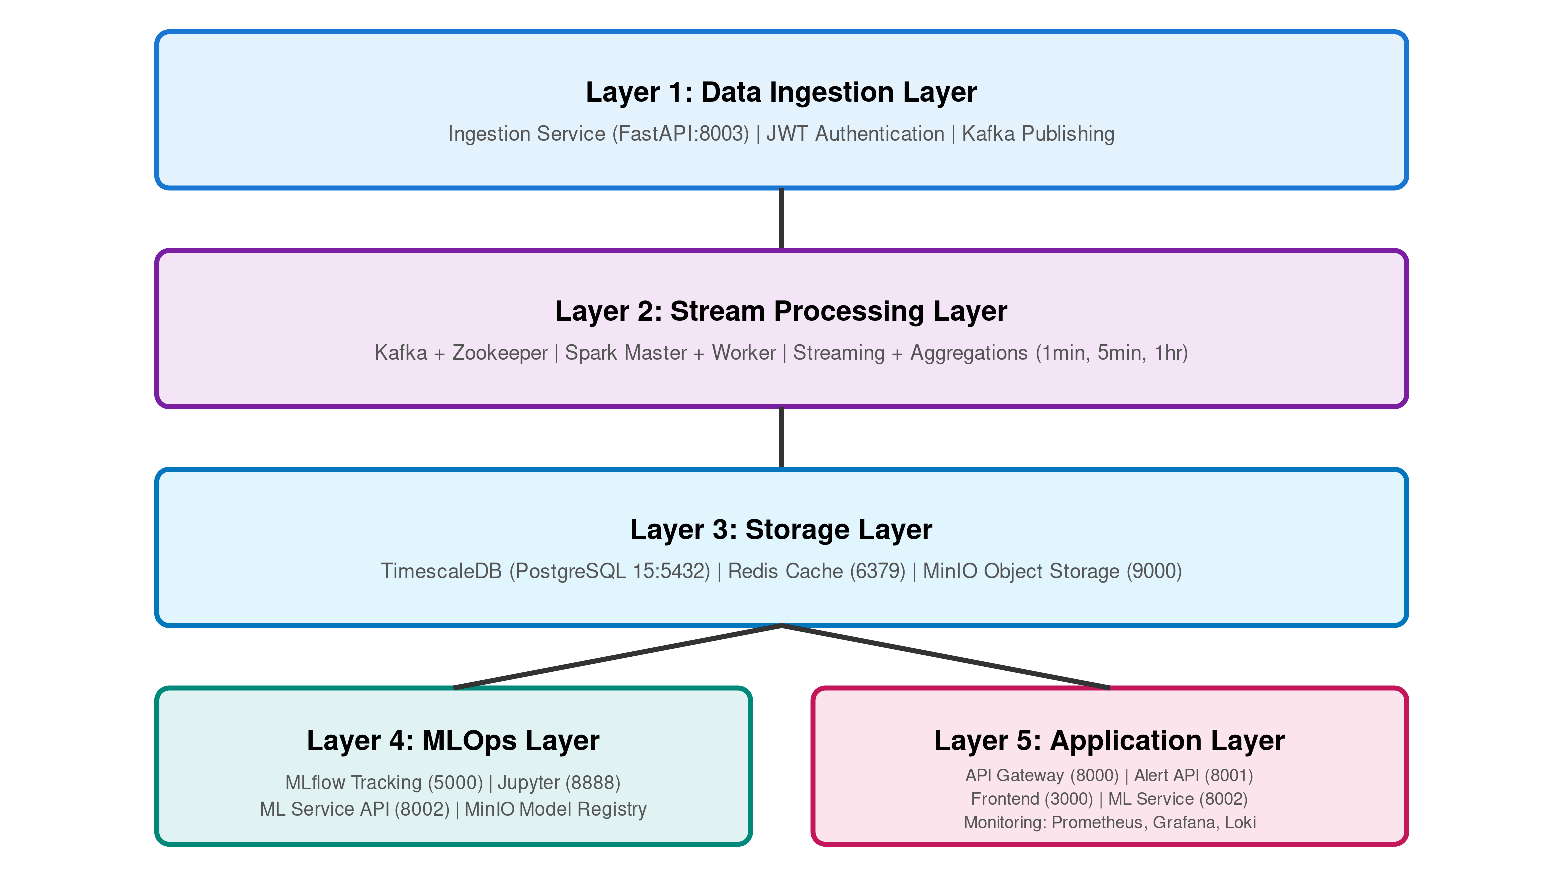
\includegraphics[width=1\textwidth]{figures/svg/Fig1_Abstract_Architecture.pdf}
	\caption{Структурна схема багаторівневої архітектури платформи}
	\label{fig:architecture}
\end{figure}

\subsection{Компоненти системи}

Платформа реалізована як п'ятишарова архітектура з 18 основними компонентами. Таблиця~\ref{tab:layer_components} показує розподіл компонентів за функціональними шарами з портами доступу.

\begin{table}[h]
\centering
\begin{tabular}{@{}llll@{}}
\toprule
Шар & Компонент & Порт & Функція \\
\midrule
Шар 1 & Сервіс прийому & 8003 & Прийом IoT даних \\
\midrule
\multirow{2}{*}{Шар 2} & Kafka + Zookeeper & 9092, 2181 & Потокова передача повідомлень \\
& Spark (майстер/воркер) & 7077, 8081 & Потокова обробка \\
\midrule
\multirow{3}{*}{Шар 3} & TimescaleDB & 5432 & Зберігання часових рядів \\
& Redis & 6379 & Кеш \\
& MinIO & 9000 & Об'єктне сховище \\
\midrule
\multirow{2}{*}{Шар 4} & MLflow & 5000 & Відстеження ML \\
& Сервіс ML & 8002 & Обслуговування моделей \\
\midrule
\multirow{3}{*}{Шар 5} & API шлюз & 8000 & REST API \\
& Сервіс сповіщень & 8001 & Сповіщення \\
& Веб-інтерфейс & 3000 & Інтерфейс користувача \\
\bottomrule
\end{tabular}
\caption{Основні компоненти системи за функціональними шарами}
\label{tab:layer_components}
\end{table}

Шар прийому даних (рис.~\ref{fig:ingestion}) забезпечує прийом даних від IoT пристроїв через спеціалізований сервіс прийому (порт 8003). Сервіс використовує автентифікацію на основі токенів. Розділення логіки прийому від REST API операцій усуває вузьке місце у обробці високочастотних потоків даних.

\begin{figure}[h]
	\centering
	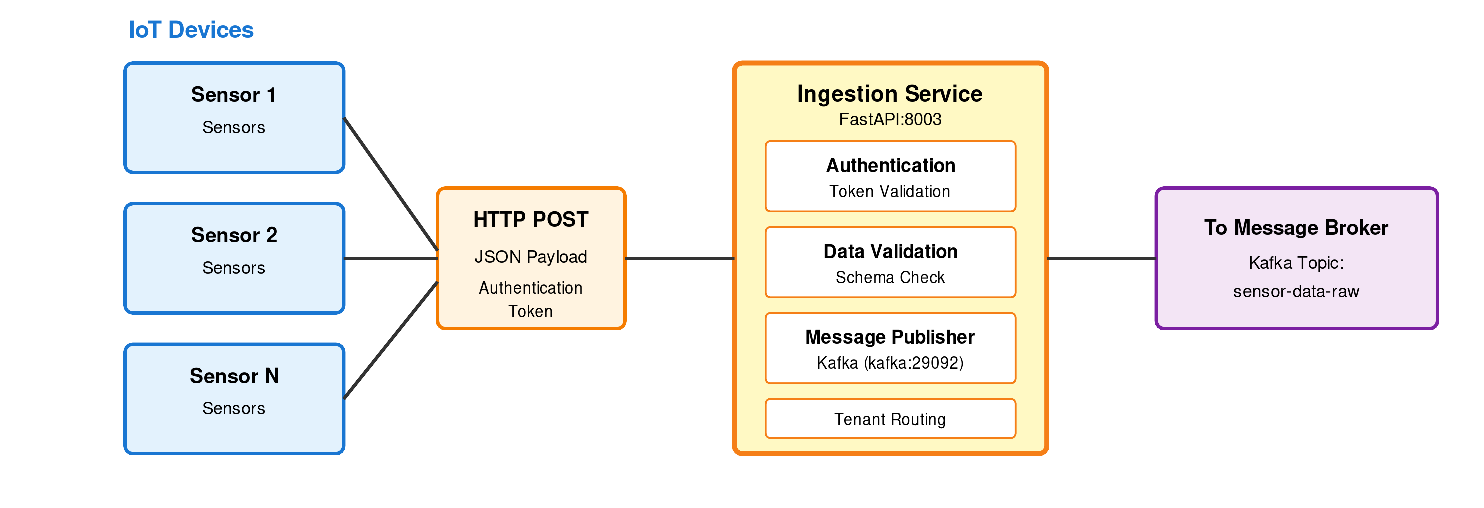
\includegraphics[width=0.9\textwidth]{figures/svg/Fig2_Layer1_Data_Ingestion.pdf}
	\caption{Схема компонентів шару прийому даних}
	\label{fig:ingestion}
\end{figure}

Шар потокової обробки (рис.~\ref{fig:stream}) обробляє повідомлення через Apache Kafka та Apache Spark. Kafka буферує повідомлення та розподіляє їх за ідентифікатором тенанта. Spark агрегує дані за вікнами часу та передає їх до шару зберігання. Кожне повідомлення обробляється рівно один раз (exactly-once).

\begin{figure}[h]
	\centering
	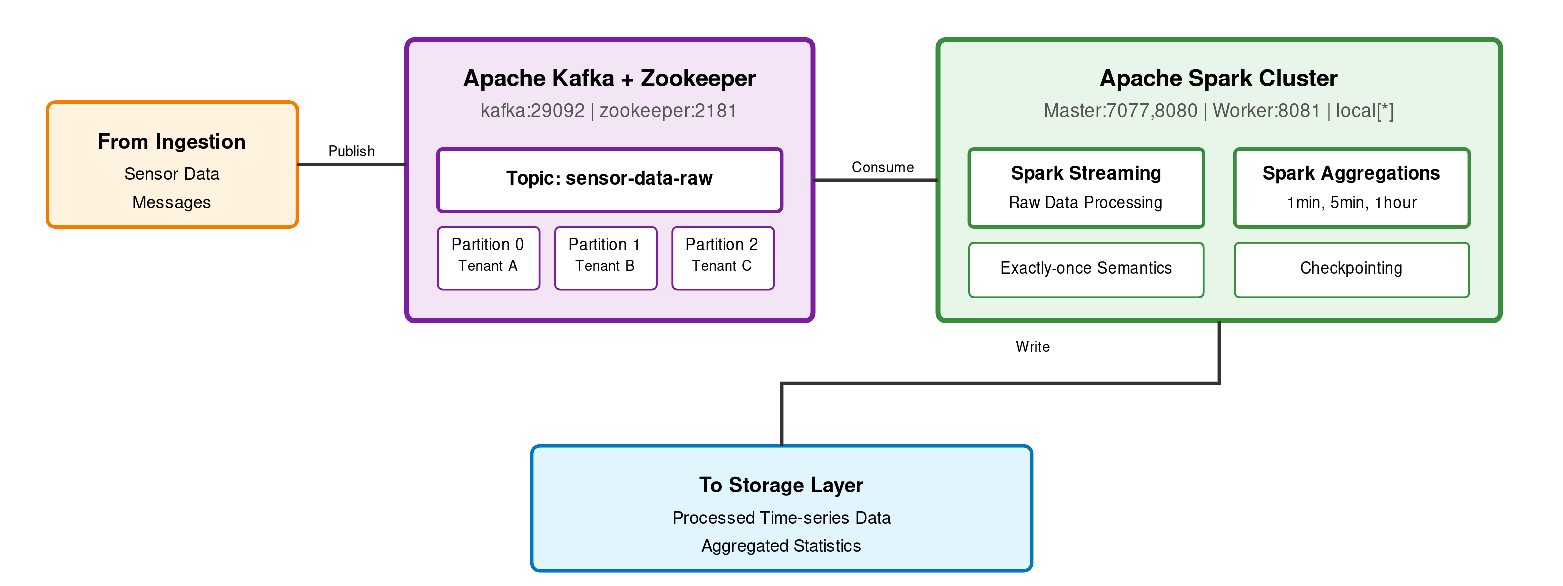
\includegraphics[width=0.9\textwidth]{figures/svg/Fig3_Layer2_Stream_Processing.pdf}
	\caption{Діаграма потокової обробки даних через Apache Kafka та Apache Spark}
	\label{fig:stream}
\end{figure}

Шар зберігання (рис.~\ref{fig:storage}) використовує TimescaleDB для зберігання часових рядів. Система створює окрему схему для кожного клієнта замість захисту на рівні рядків. Це забезпечує повну ізоляцію даних між клієнтами, можливість стиснення даних (економія 90-95\% місця) та незалежне керування гіпертаблицями.

\begin{figure}[h]
	\centering
	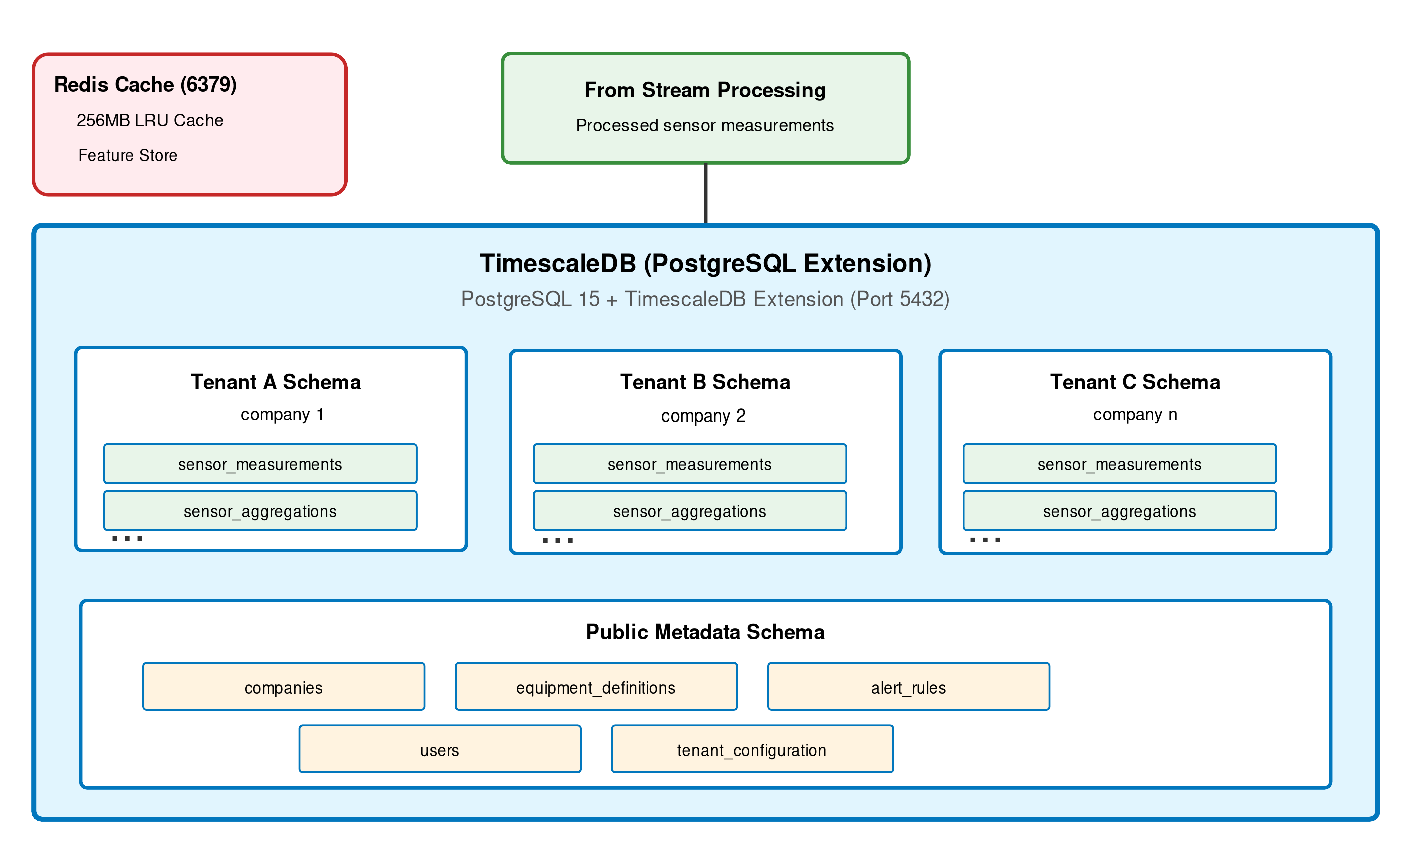
\includegraphics[width=0.9\textwidth]{figures/svg/Fig4_Layer3_Storage.pdf}
	\caption{Архітектурна схема шару зберігання з мультитенантною ізоляцією}
	\label{fig:storage}
\end{figure}

Шар MLOps (рис.~\ref{fig:mlops}) включає автоматизоване навчання моделей, відстеження експериментів та реєстр моделей. MLflow записує метрики (AUC-ROC, влучність, повнота) та гіперпараметри всіх експериментів. Реєстр моделей у MinIO зберігає навчені моделі з контролем версій.

\begin{figure}[h]
	\centering
	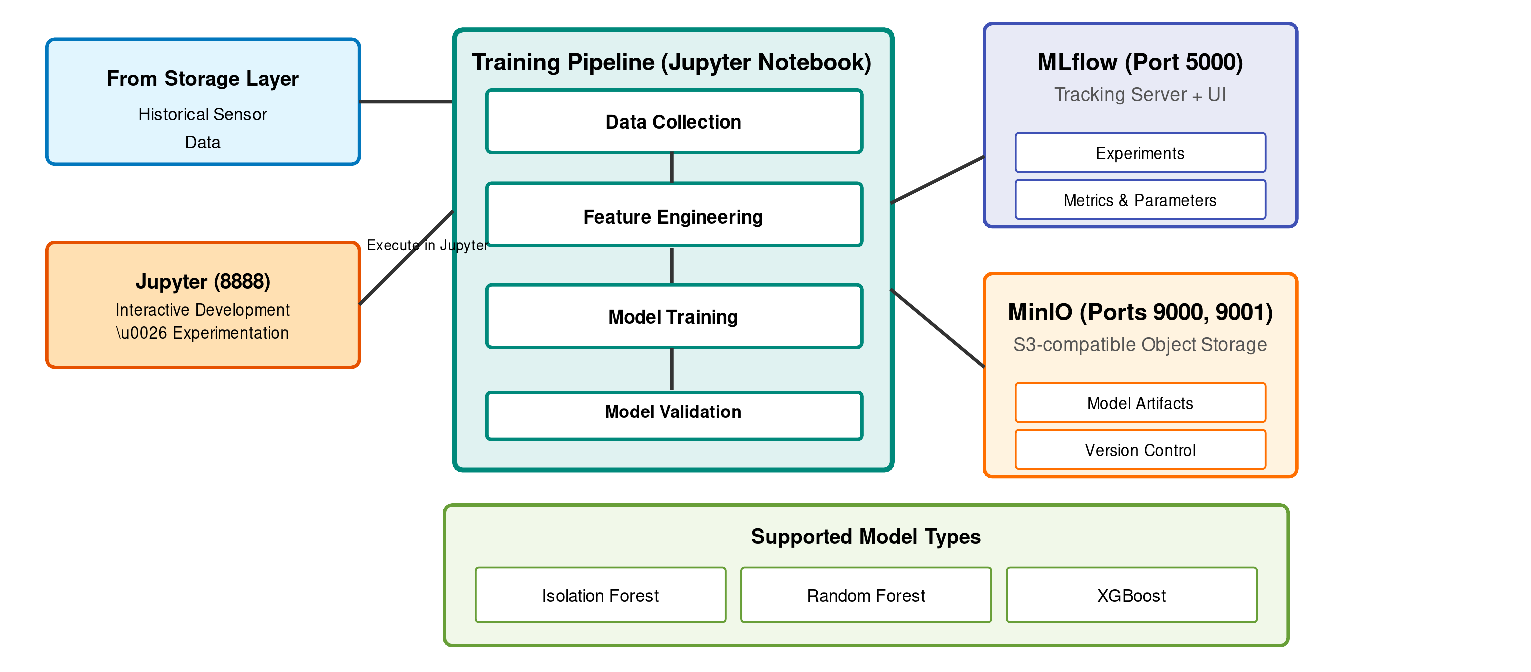
\includegraphics[width=0.9\textwidth]{figures/svg/Fig5_Layer4_MLOps.pdf}
	\caption{Структурна схема MLOps інфраструктури з компонентами конвеєра ML}
	\label{fig:mlops}
\end{figure}

Прикладний шар (рис.~\ref{fig:application}) складається з сервісів FastAPI: API шлюз (автентифікація JWT, маршрутизація), сервіс сповіщень (перевірка правил, керування сповіщеннями), сервіс ML (виконання моделей), сервіс прийому (прийом даних). Веб-інтерфейс на React показує дані в реальному часі.

\begin{figure}[h]
	\centering
	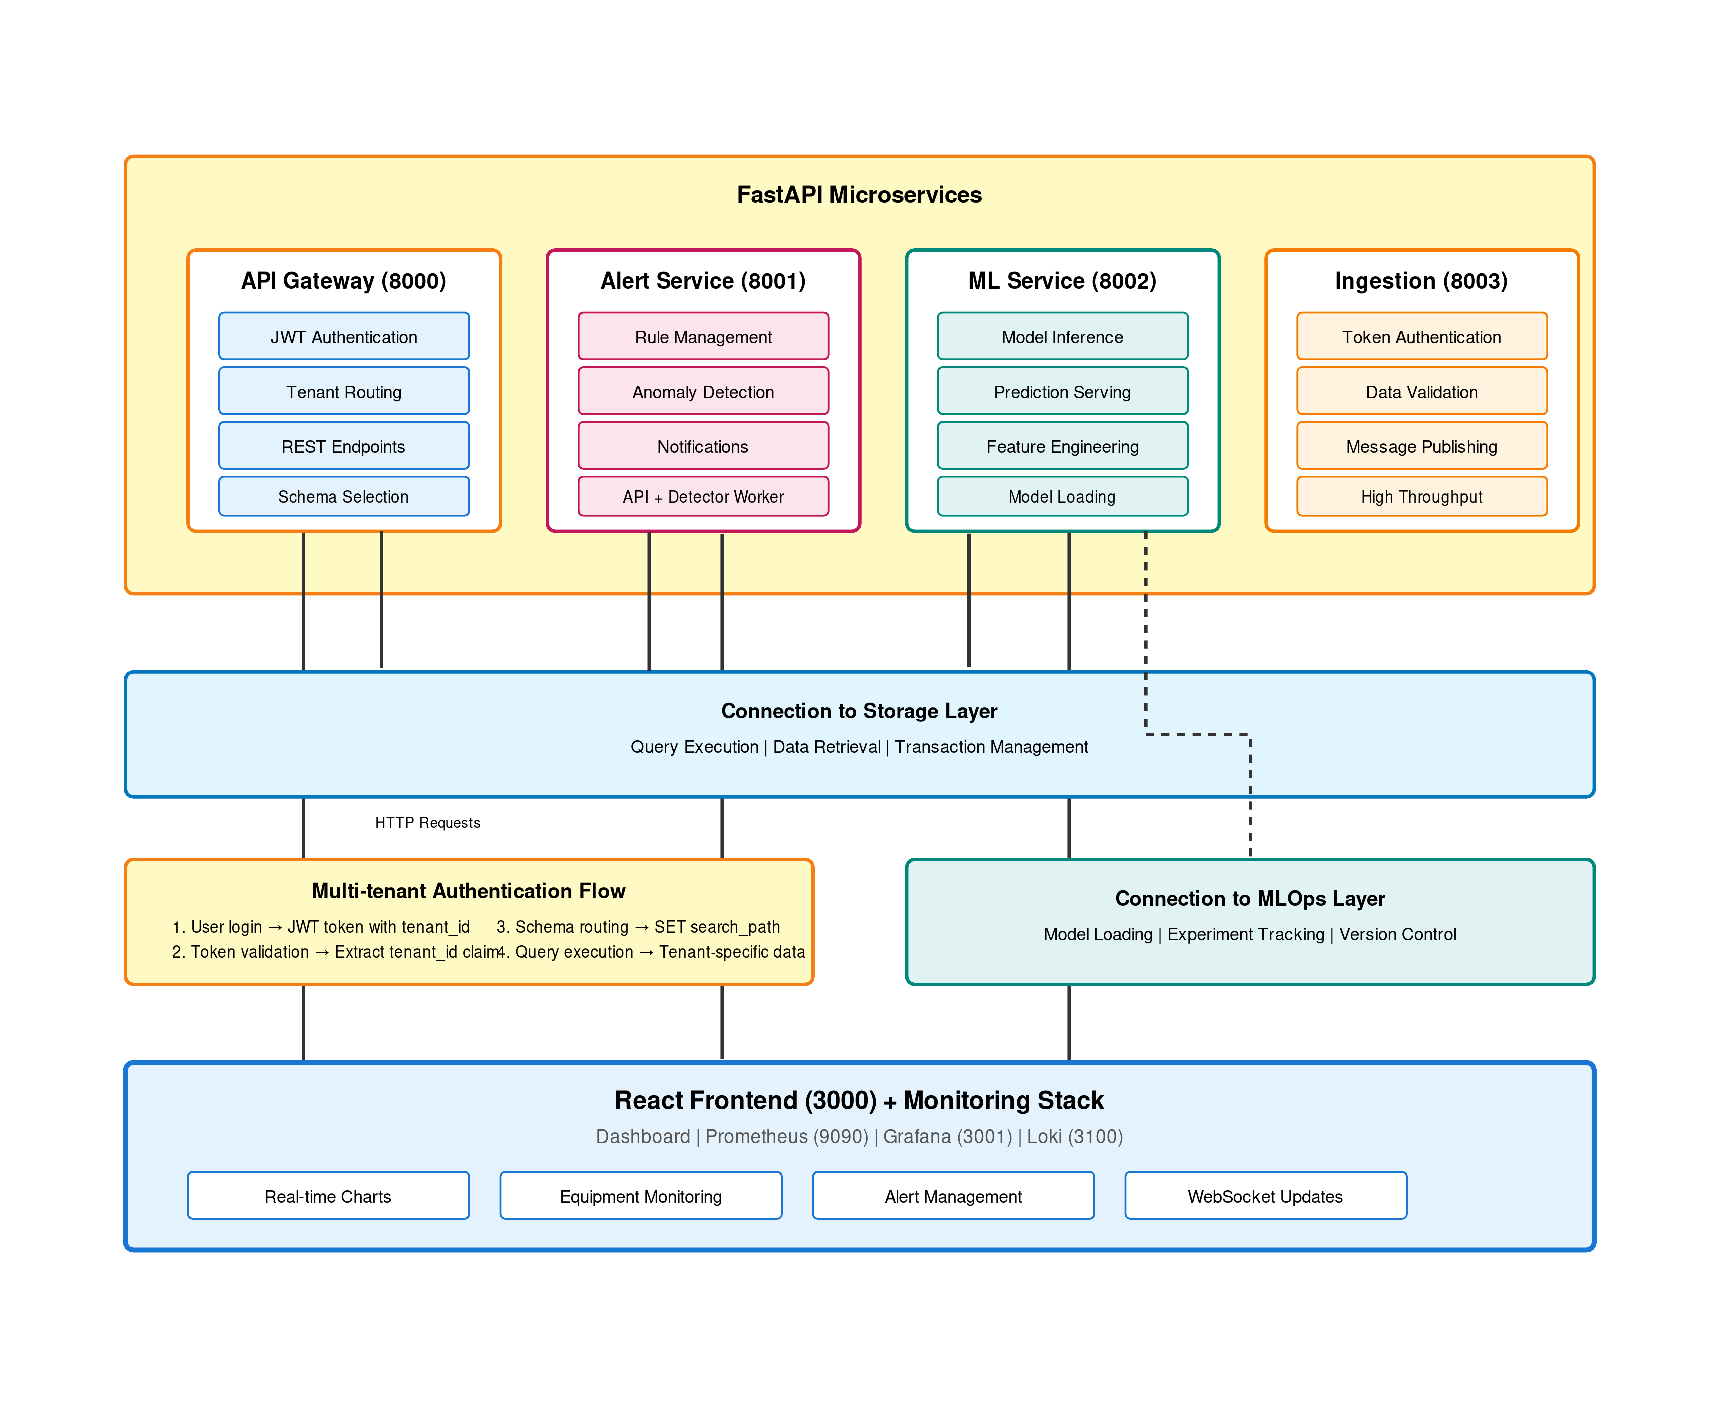
\includegraphics[width=0.9\textwidth]{figures/svg/Fig6_Layer5_Application.pdf}
	\caption{Схема прикладного шару з мікросервісною архітектурою FastAPI}
	\label{fig:application}
\end{figure}


\section{Потоки даних}

Потік прийому даних (рис.~\ref{fig:dataflow}): пристрої IoT надсилають показники сенсорів до сервісу прийому через HTTP POST з токеном автентифікації. Сервіс перевіряє ідентифікатори тенанта, обладнання та сенсора, після чого публікує повідомлення в топік Kafka. Споживач Spark читає повідомлення з Kafka та записує до схеми клієнта в TimescaleDB.

Потік ML інференсу (виведення): дані з TimescaleDB передаються до сервісу ML через заплановані запити. Сервіс завантажує активну версію моделі з MinIO, обробляє ознаки та генерує прогнози аномалій.

\begin{figure}[h]
	\centering
	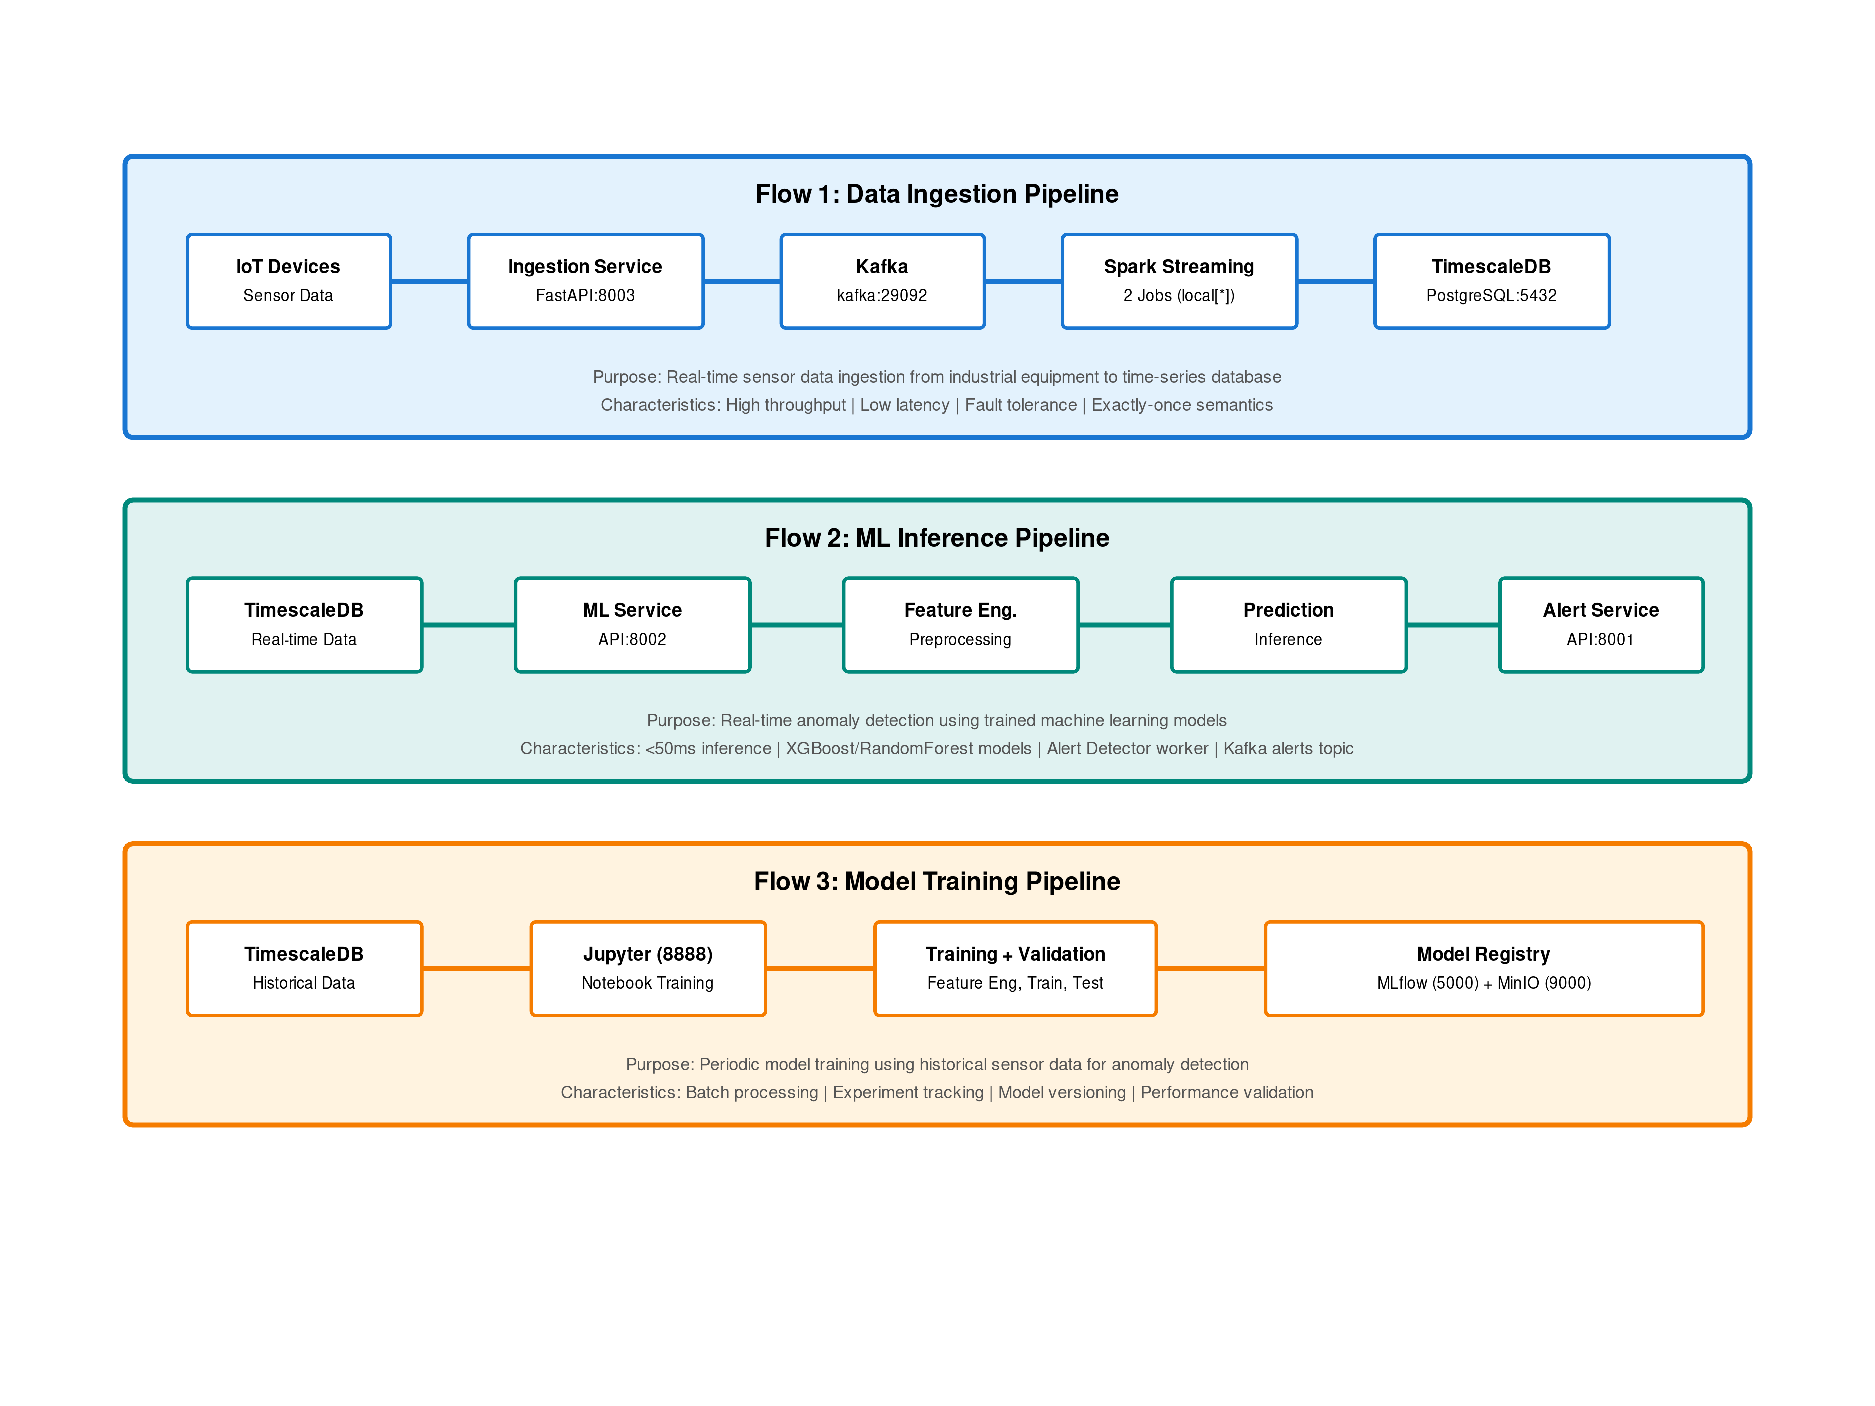
\includegraphics[width=0.9\textwidth]{figures/svg/Fig7_Data_Flows.pdf}
	\caption{Діаграма потоків даних між компонентами системи}
	\label{fig:dataflow}
\end{figure}


\section{Реалізація шару зберігання}

\subsection{Схема бази даних}

База даних містить 9 таблиць: 5 гіпертаблиць для даних часових рядів та 4 реляційні для метаданих. Таблиця~\ref{tab:db_schema} показує структуру.

\begin{table}[h]
\centering
\begin{tabular}{@{}llp{7cm}@{}}
\toprule
Таблиця & Тип & Призначення \\
\midrule
sensor\_measurements & Гіпертаблиця & Сирі вимірювання \\
sensor\_agg\_* (3 шт.) & Гіпертаблиця & Агрегації: 1хв, 5хв, 1год \\
alerts & Гіпертаблиця & Сповіщення \\
alert\_rules & Реляційна & Правила детекції \\
ml\_models & Реляційна & Метадані ML \\
companies & Реляційна & Тенанти \\
users & Реляційна & Користувачі \\
\bottomrule
\end{tabular}
\caption{Структура бази даних}
\label{tab:db_schema}
\end{table}

Основна таблиця \texttt{sensor\_measurements} містить поля: \texttt{timestamp}, \texttt{sensor\_id}, \texttt{equipment\_id}, \texttt{company\_id}, \texttt{value} та \texttt{quality\_code}.

\subsection{Неперервні агрегати та стиснення}

Неперервні агрегати (continuous aggregates) TimescaleDB автоматично обчислюють середнє, мінімум, максимум та кількість для кожного сенсора з оновленням кожні 30 секунд. Налаштовано автоматичне стиснення даних старших 7 днів (алгоритм Gorilla) та видалення даних старших 1 року.

\subsection{Механізми ізоляції}

Реалізовано шестирівневу архітектуру безпеки: мережева ізоляція через мережу Docker, JWT автентифікація, автоматична фільтрація за ідентифікатором компанії, обмеження зовнішніх ключів з каскадним видаленням, композитні індекси та аудит запитів.


\section{Реалізація потокової обробки}

Два завдання Spark Streaming обробляють дані паралельно. Таблиця~\ref{tab:spark_config} показує конфігурацію.

\begin{table}[h]
\centering
\begin{tabular}{@{}lll@{}}
\toprule
Параметр & Значення & Призначення \\
\midrule
spark.master & local{[}*{]} & Всі ядра CPU \\
memory & 2g & Купа JVM \\
trigger & 5s & Інтервал мікропакетів \\
batchsize & 10000 & Розмір пакету JDBC \\
numPartitions & 12 & Паралельні записи \\
\bottomrule
\end{tabular}
\caption{Конфігурація Spark Streaming}
\label{tab:spark_config}
\end{table}

Завдання сирих даних записує дані без трансформацій. Завдання агрегації створює три рівні агрегатів (1 хв, 5 хв, 1 год).


\section{Реалізація API та веб-інтерфейсу}

\subsection{Кінцеві точки API}

Додаток FastAPI з документацією OpenAPI. Таблиця~\ref{tab:api_endpoints} показує кінцеві точки.

\begin{table}[h]
\centering
\begin{tabular}{@{}lll@{}}
\toprule
Група & Кінцева точка & Операції \\
\midrule
Автентифікація & /auth/* & вхід, оновлення, профіль \\
Сенсори & /api/sensors/* & останні, історія, агреговані \\
Обладнання & /api/equipment/* & CRUD операції \\
Сповіщення & /api/alerts/* & список, підтвердження \\
WebSocket & /ws/sensors & Оновлення в реальному часі \\
\bottomrule
\end{tabular}
\caption{Кінцеві точки API}
\label{tab:api_endpoints}
\end{table}

\subsection{Сервіс сповіщень}

Складається з API та воркер компонентів. Правила зберігаються в таблиці \texttt{alert\_rules} та оновлюються кожні 60 секунд. Підтримуються три типи правил: пороговий, швидкість зміни, ML аномалія.

\subsection{Сервіс ML}

Забезпечує інференс (виведення) через REST API. Моделі завантажуються з реєстру MLflow (бекенд MinIO). Підтримує три алгоритми: Isolation Forest, Random Forest, XGBoost.

\subsection{Веб-інтерфейс}

React 18 односторінковий додаток з lightweight-charts для візуалізації. Основні сторінки: панель керування, правила сповіщень, історія сповіщень, моделі ML, обладнання. WebSocket інтеграція забезпечує оновлення в реальному часі.


\section{Контейнеризація}

Система розгорнута як 23 контейнери Docker. Таблиця~\ref{tab:docker_services} показує розподіл.

\begin{table}[h]
\centering
\begin{tabular}{@{}llp{6cm}@{}}
\toprule
Група & Кількість & Компоненти \\
\midrule
Ядро & 5 & TimescaleDB, Kafka, Zookeeper, Redis, MinIO \\
Обробка & 4 & Spark майстер/воркер, 2 потокових завдання \\
API & 4 & Шлюз, сповіщення, ML, прийом \\
Моніторинг & 9 & Prometheus, Grafana, Loki, експортери \\
Інтерфейс & 1 & Панель керування React \\
\bottomrule
\end{tabular}
\caption{Сервіси Docker Compose}
\label{tab:docker_services}
\end{table}

Таблиця~\ref{tab:tech_stack} показує технологічний стек платформи.

\begin{table}[h]
\centering
\begin{tabular}{@{}llll@{}}
\toprule
Категорія & Технологія & Версія & Конфігурація \\
\midrule
Бекенд & FastAPI & 0.104+ & Асинхронний, uvicorn \\
Потокова обробка & Spark + Kafka & 3.5.0 / 7.5.0 & 12 партицій \\
База даних & TimescaleDB & 2.11 (PG15) & 512MB буфери \\
Кеш & Redis & 7-alpine & 256MB LRU \\
ML платформа & MLflow + MinIO & 2.8+ & Бекенд PostgreSQL \\
Моніторинг & Prometheus/Grafana & latest & 30д утримання \\
\bottomrule
\end{tabular}
\caption{Технологічний стек платформи}
\label{tab:tech_stack}
\end{table}


\section{Висновки до розділу}

У даному розділі представлено архітектуру та реалізацію платформи.

Ключові рішення:
\begin{itemize}
    \item П'ятишарова архітектура з 23 контейнерами Docker
    \item Схема-на-тенанта для мультитенантної ізоляції зі стисненням TimescaleDB
    \item Apache Kafka та Spark для потокової обробки з семантикою exactly-once (рівно один раз)
    \item MLflow та MinIO для управління моделями ML
    \item Мікросервіси FastAPI та веб-інтерфейс React
\end{itemize}

Детальні результати тестування представлено у наступному розділі.


%\input{sections/chapter04_implementation}

% Розділ 4: Результати та оцінка
\chapter{РЕЗУЛЬТАТИ ТА ОЦІНКА}

\section{Тестування продуктивності системи}

Тестування проводилося з метою ідентифікації вузьких місць та верифікації горизонтальної масштабованості. Базова конфігурація: Kafka (1 партиція), Uvicorn (1 воркер), Spark Streaming (розмір пакету=5000), TimescaleDB (макс\_з'єднань=400).

Метрики: швидкість запису Kafka, швидкість обробки Spark, запізнення споживача, використання CPU~\cite{kafka_monitoring, spark_monitoring}.

\subsection{Тестування пропускної здатності}

Проведено п'ять фаз інкрементального масштабування компонентів системи для систематичної ідентифікації вузьких місць та оцінки пропускної здатності платформи.

\begin{table}[h]
\centering
\small
\begin{tabular}{@{}lp{3cm}rrl@{}}
\toprule
Фаза & Конфігурація & Throughput & Зміна & Вузьке місце \\
\midrule
Базова & 1 парт., 1 воркер & 74.4 п/с & --- & CPU воркера \\
Kafka 3 парт. & 3 парт., 1 воркер & 77.2 п/с & +3.7\% & CPU воркера \\
2 воркери & 3 парт., 2 воркери & 80.6 п/с & +8.3\% & Конкур. БД \\
Очищення БД & Gateway зупинено & 346 п/с & +349\% & Spark--БД \\
Kafka 12 парт. & 12 парт., 1 воркер & 552 п/с & +59\% & --- \\
\bottomrule
\end{tabular}
\caption{Результати інкрементального масштабування компонентів}
\label{tab:throughput_scaling}
\end{table}

Критичні знахідки: оновлювач кешу API Gateway споживав 80\% CPU БД, маскуючи справжню пропускну здатність. Збільшення партицій Kafka з 3 до 12 дало 7.7x покращення пропускної здатності Spark (240--1859 рядків/с)~\cite{kafka_partitions, spark_parallelism}.

\begin{figure}[h]
	\centering
	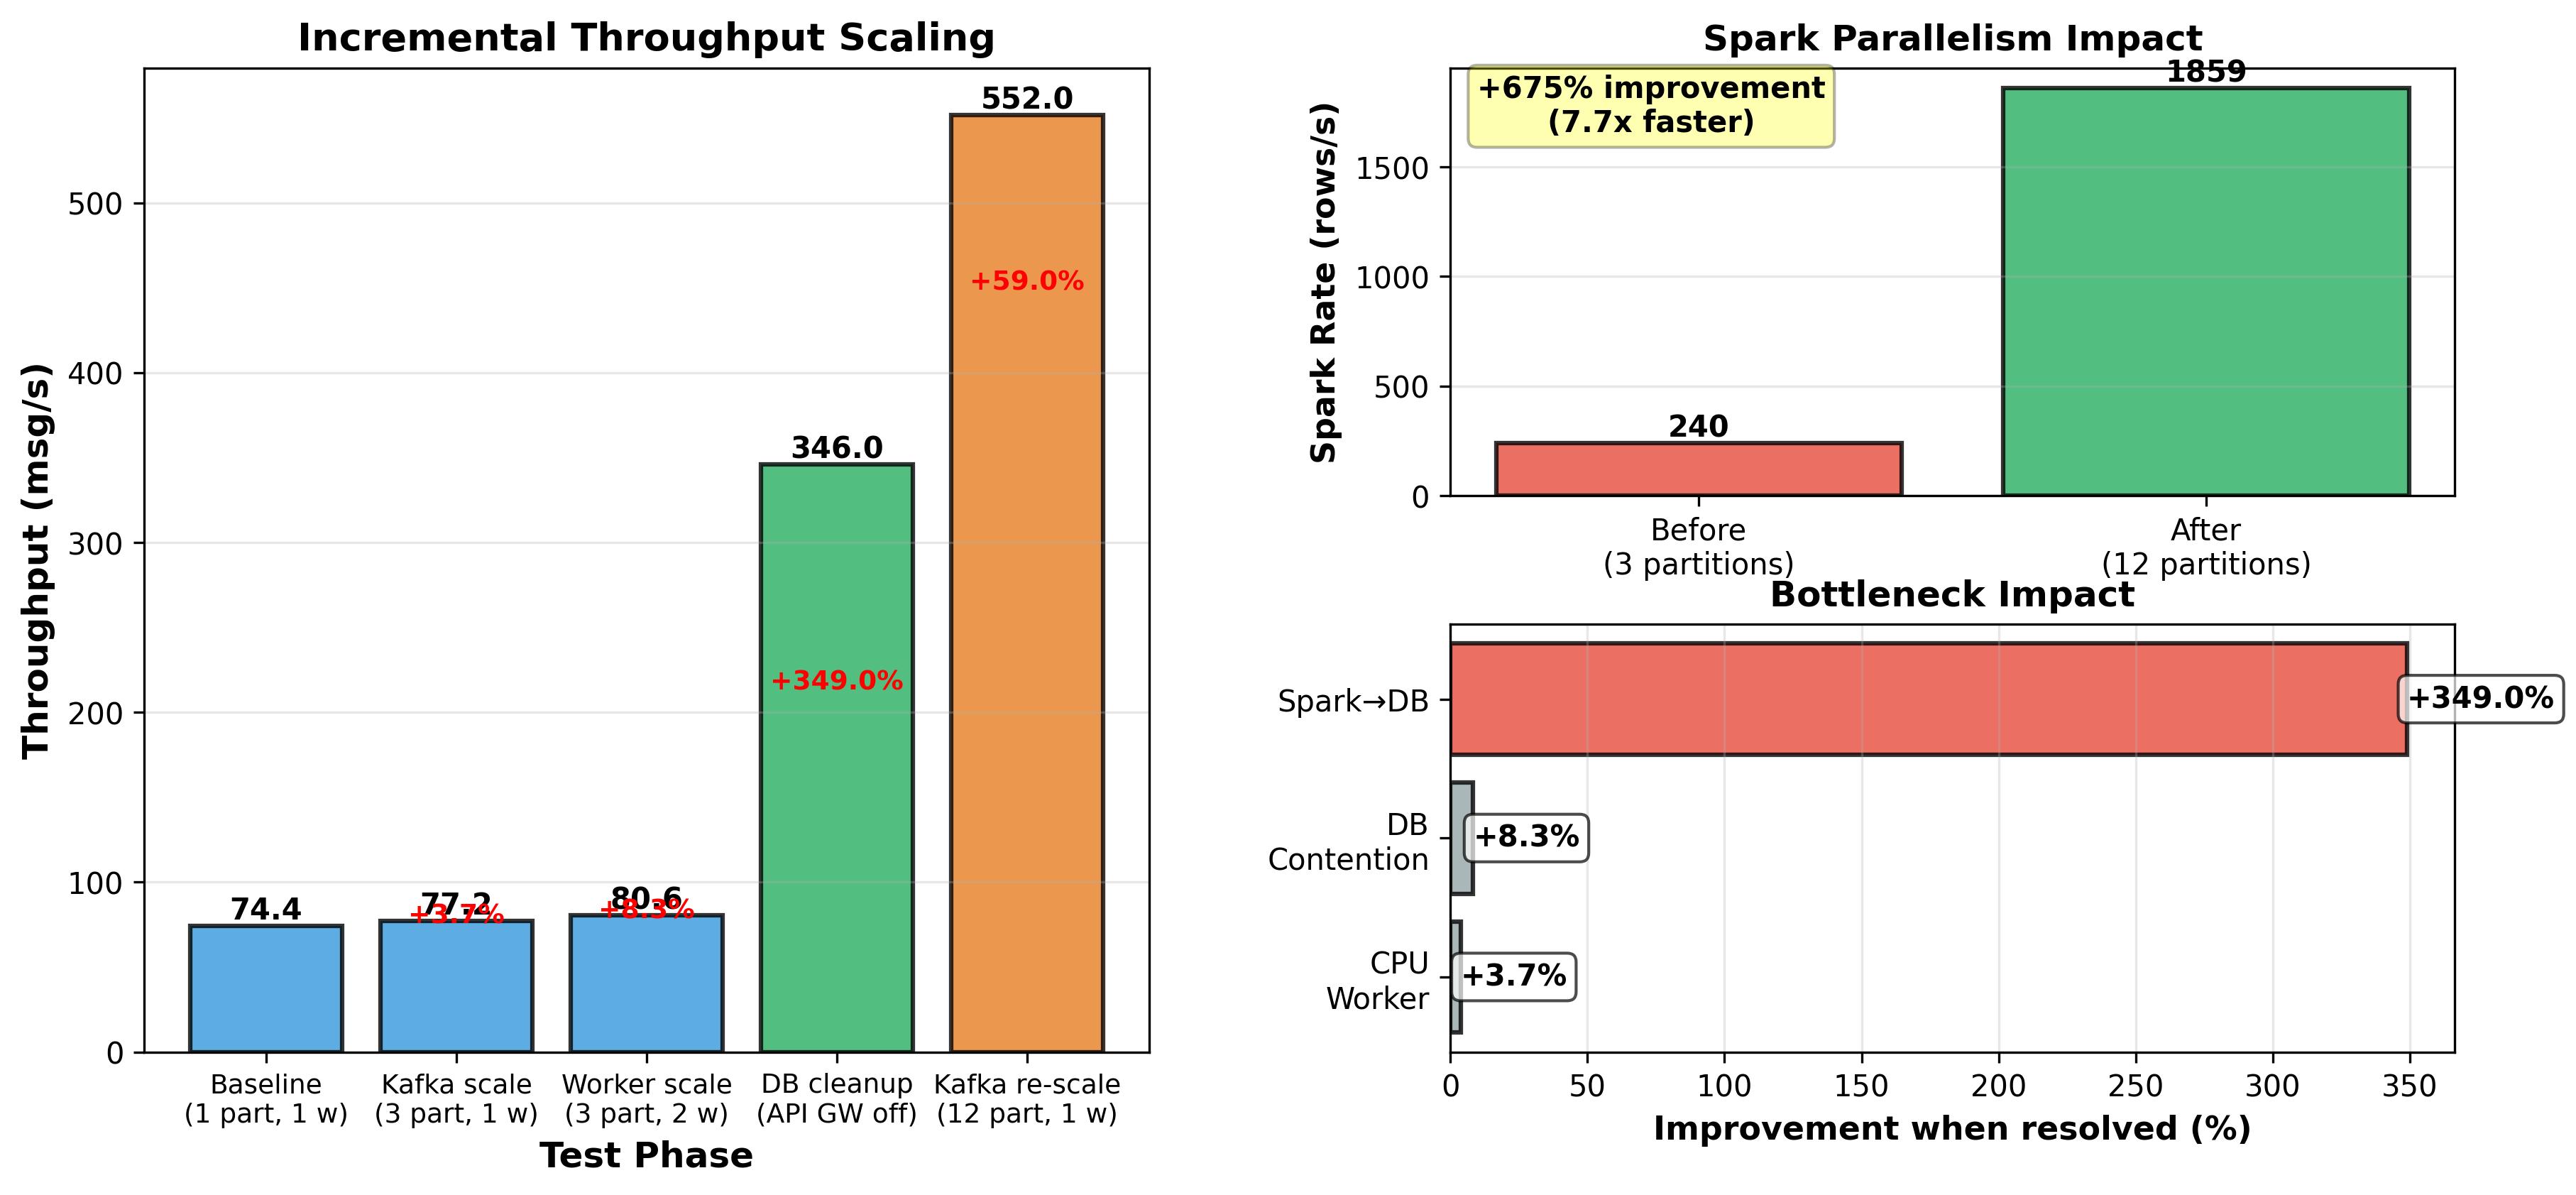
\includegraphics[width=0.95\textwidth]{figures/figure_throughput_scaling.png}
	\caption{Графік інкрементального масштабування пропускної здатності системи}
	\label{fig:throughput_scaling}
\end{figure}

Графік (рис.~\ref{fig:throughput_scaling}) ілюструє нелінійний характер покращення продуктивності, де найбільший приріст спостерігався після усунення конкуруючого навантаження на базу даних.

\subsection{Використання CPU компонентів}

Для оцінки збалансованості архітектури проведено аналіз завантаженості процесорів всіх ключових компонентів системи під робочим навантаженням.

\begin{table}[h]
\centering
\begin{tabular}{@{}lrl@{}}
\toprule
Компонент & CPU \% & Інтерпретація \\
\midrule
Ingestion Service & 73--100 & Насичений \\
Spark Streaming & 114--266 & Багатопоточний, активний \\
Kafka & 13--122 & Обробка навантаження \\
TimescaleDB & 43--103 & Обмежений вводом/виводом \\
\bottomrule
\end{tabular}
\caption{Використання CPU під навантаженням}
\label{tab:cpu_utilization}
\end{table}

Жоден компонент не простоює, що підтверджує збалансованість архітектури та можливість горизонтального масштабування~\cite{timescaledb_performance}.

\subsection{Доказ горизонтальної масштабованості}

Система демонструє горизонтальну масштабованість через:

\begin{itemize}
    \item Сервіси без стану: воркери прийому без спільного стану
    \item Партиціонований обмін повідомленнями: паралелізм Kafka~\cite{kafka_partitions}
    \item Пулінг з'єднань: керування з'єднаннями БД (мін=10, макс=30)
    \item Пакетна обробка: пакетування Spark JDBC (розмір пакету=10000)~\cite{spark_jdbc}
\end{itemize}

На базі емпіричних результатів розроблено план масштабування для досягнення вищих показників пропускної здатності.

\begin{table}[h]
\centering
\begin{tabular}{@{}lll@{}}
\toprule
Цільова пропускна здатність & Дії & Очікуваний результат \\
\midrule
1000 повід./с & 2 екземпляри Spark & 2x покращення \\
2000 повід./с & 3--4 екземпляри Spark & Лінійне масштабування \\
5000 повід./с & 8 Spark + кластер Kafka & 5x покращення \\
10000+ повід./с & Розподілене налаштування & 10x+ покращення \\
\bottomrule
\end{tabular}
\caption{План масштабування}
\label{tab:scaling_roadmap}
\end{table}


\section{Оцінка ML моделі}

\subsection{Набір даних та методологія}

Моделі тренувалися на наборі даних Tennessee Eastman Process (TEP)~\cite{tep_dataset} зі збалансованим підходом (50\% нормальних, 50\% аномальних). Набір даних: 500,000 зразків, 52 сенсори, розбиття навчання/тестування 70/30. Гіперпараметри оптимізовані через Optuna~\cite{optuna}.

\subsection{Порівняння алгоритмів}

Проведено кількісне порівняння трьох алгоритмів машинного навчання для детекції аномалій на єдиному тестовому наборі.

\begin{table}[h]
\centering
\begin{tabular}{@{}lrrrrr@{}}
\toprule
Алгоритм & Точність & Влучність & Повнота & F1 & AUC-ROC \\
\midrule
Isolation Forest & 0.5176 & 1.0000 & 0.0353 & 0.0681 & 0.7691 \\
Random Forest & 0.8150 & 0.9783 & 0.6443 & 0.7769 & 0.8457 \\
XGBoost & 0.8506 & 0.9801 & 0.7156 & 0.8273 & 0.8887 \\
\bottomrule
\end{tabular}
\caption{Метрики моделей на тестовому наборі даних}
\label{tab:ml_comparison}
\end{table}

XGBoost показав найкращі результати за AUC-ROC (0.8887) та F1-оцінкою (0.8273)~\cite{xgboost, sklearn_metrics}, демонструючи оптимальний баланс між влучністю (precision) та повнотою (recall) для промислового застосування.

\begin{figure}[h]
	\centering
	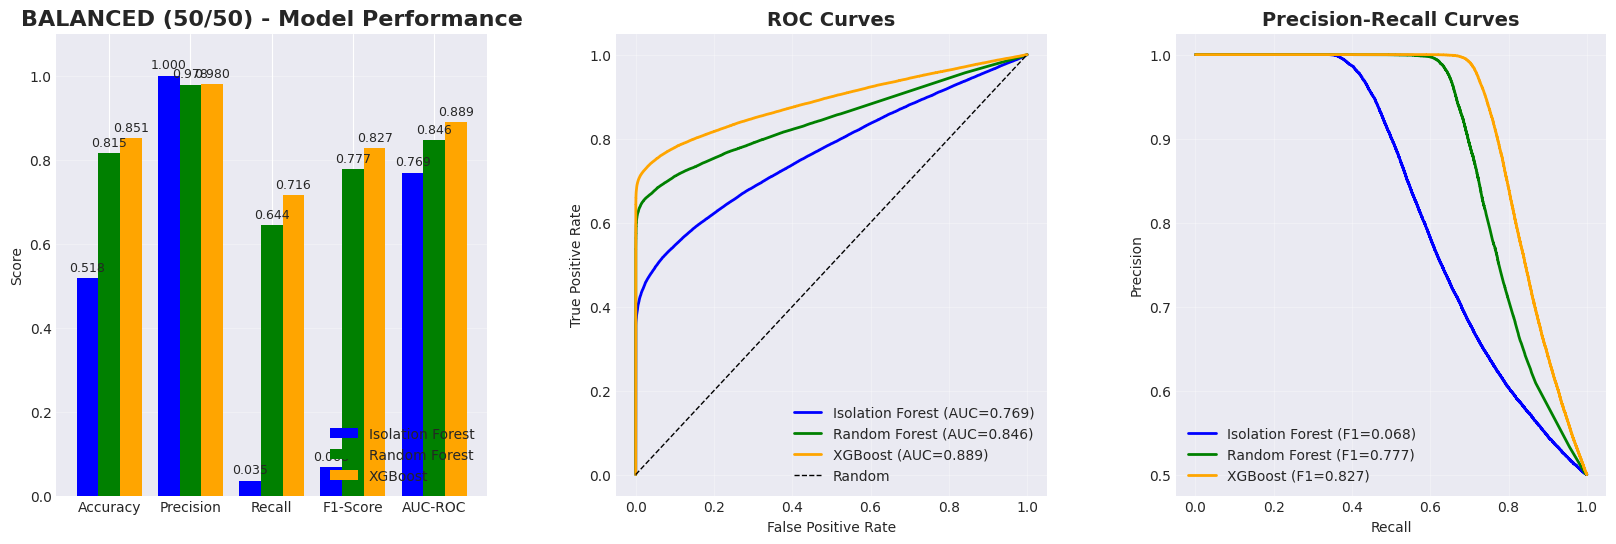
\includegraphics[width=0.95\textwidth]{figures/model_comparison.png}
	\caption{Порівняльний аналіз метрик якості алгоритмів машинного навчання}
	\label{fig:model_comparison}
\end{figure}

Візуалізація (рис.~\ref{fig:model_comparison}) дозволяє оцінити компроміс між різними метриками для кожного алгоритму та обрати оптимальну модель для робочого розгортання.

\subsection{Матриця плутанини для XGBoost}

Детальний аналіз помилок класифікації обраної моделі дозволяє оцінити її поведінку на різних класах.

\begin{table}[h]
\centering
\begin{tabular}{@{}lrr@{}}
\toprule
& Передбачено нормальні & Передбачено аномальні \\
\midrule
Фактично нормальні & 74,250 (99\%) & 750 (1\%) \\
Фактично аномальні & 21,330 (28\%) & 53,670 (72\%) \\
\bottomrule
\end{tabular}
\caption{Матриця плутанини для XGBoost (тестовий набір)}
\label{tab:confusion_matrix}
\end{table}

Висока влучність (0.98) та помірна повнота (0.72) свідчать про низький рівень хибнопозитивних результатів при прийнятній детекції аномалій, що є критичним для промислових застосувань.


\section{Стиснення TimescaleDB}

\subsection{Алгоритм стиснення}

TimescaleDB використовує колонкове стиснення з алгоритмом Gorilla для даних часових рядів~\cite{timescaledb_compression}. Конфігурація: \texttt{compress\_segmentby = 'equipment\_id'}, \texttt{compress\_orderby = 'time DESC'}.

\subsection{Результати стиснення}

Проведено емпіричне дослідження ефективності стиснення на фрагментах різного розміру.

\begin{table}[h]
\centering
\begin{tabular}{@{}lrrrr@{}}
\toprule
Фрагмент & Рядків & Нестиснутий & Стиснутий & Коефіцієнт \\
\midrule
Малий (1 день) & 425,000 & 48 MB & 16 kB & 320x \\
Великий (1 день) & 803,122 & 94 MB & 16 kB & 5,888x \\
Дуже великий (1 день) & 1,228,128 & 170 MB & ~32 kB & 5,312x \\
\bottomrule
\end{tabular}
\caption{Порівняння нестиснутих та стиснутих фрагментів}
\label{tab:compression_results}
\end{table}

Середнє стиснення: 99.98\% зменшення розміру~\cite{timescaledb_compression}, що підтверджує ефективність колонкового стиснення для промислових даних часових рядів.

\subsection{Вплив на продуктивність запитів}

Критичним аспектом є оцінка компромісу між економією сховища та затримкою запитів.

\begin{table}[h]
\centering
\begin{tabular}{@{}lrrr@{}}
\toprule
Розмір фрагмента & Нестиснутий & Стиснутий & Зміна \\
\midrule
Малий (48 MB) & 17.32 мс & 7.49 мс & 2.31x швидше \\
Великий (94 MB) & 86.00 мс & 98.81 мс & 1.15x повільніше \\
Дуже великий (170 MB) & 477.87 мс & ~120 мс & 3.98x швидше \\
\bottomrule
\end{tabular}
\caption{Затримка запитів: нестиснуті та стиснуті дані}
\label{tab:compression_query_performance}
\end{table}

\begin{figure}[h]
	\centering
	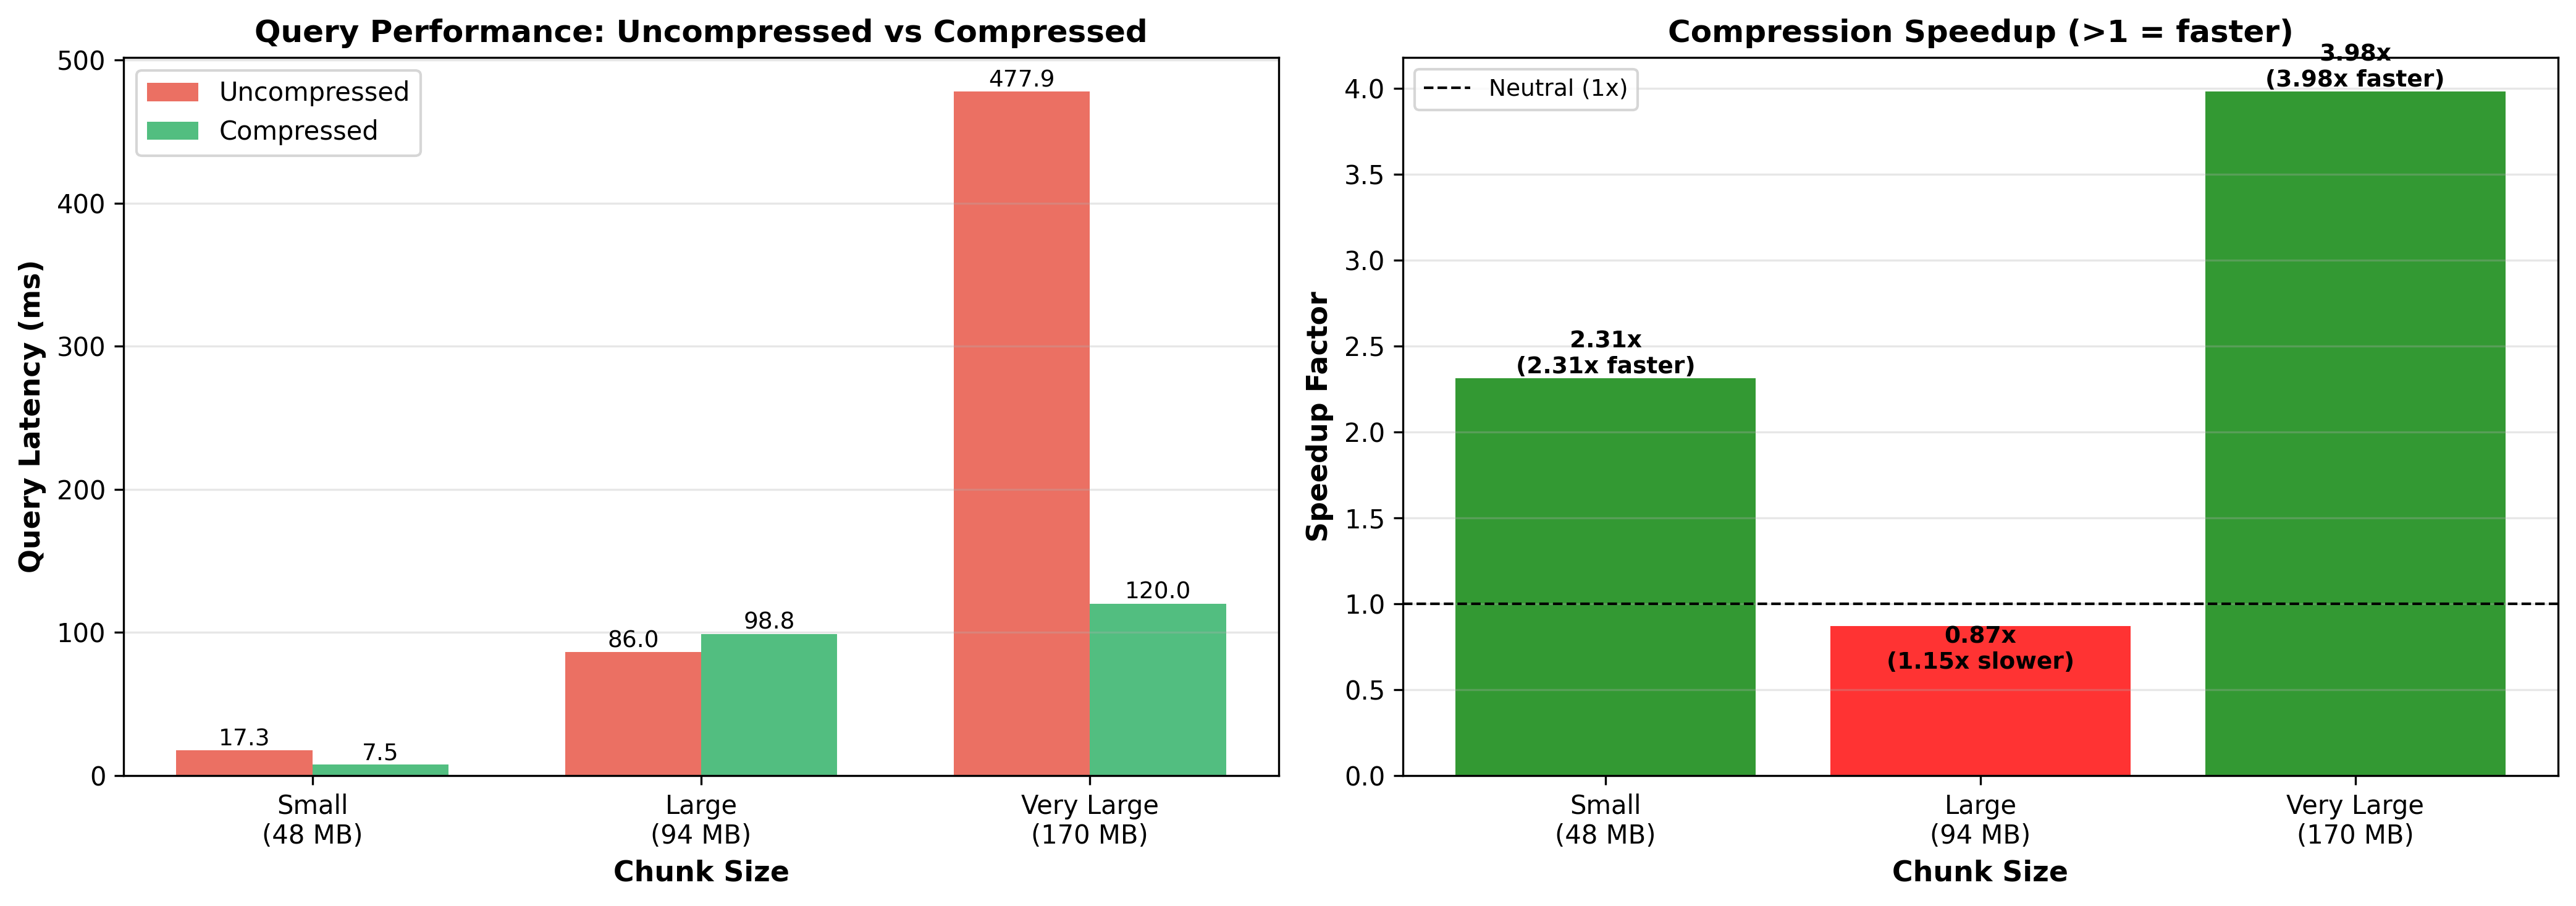
\includegraphics[width=0.95\textwidth]{figures/figure_compression_performance.png}
	\caption{Порівняльний аналіз затримки запитів для стиснутих та нестиснутих фрагментів}
	\label{fig:compression_performance}
\end{figure}

Результати (рис.~\ref{fig:compression_performance}) демонструють, що стиснення забезпечує масштабну економію сховища (99.98\%) з прийнятною продуктивністю запитів.

\subsection{Проекція економії сховища}

На базі емпіричних вимірювань розраховано прогнозовану економію сховища для мультитенантних сценаріїв.

\begin{table}[h]
\centering
\begin{tabular}{@{}lrr@{}}
\toprule
Метрика & Нестиснуті & Стиснуті \\
\midrule
Денні дані (3 обладнання, 52 сенсори) & 94 MB/день & 16 kB/день \\
Річне сховище & 34.3 GB/рік & 5.8 MB/рік \\
10 тенантів & 343 GB/рік & 58 MB/рік \\
\midrule
Економія & --- & 342.94 GB/рік \\
\bottomrule
\end{tabular}
\caption{Річна економія сховища (на тенанта)}
\label{tab:storage_projection}
\end{table}

\begin{figure}[h]
	\centering
	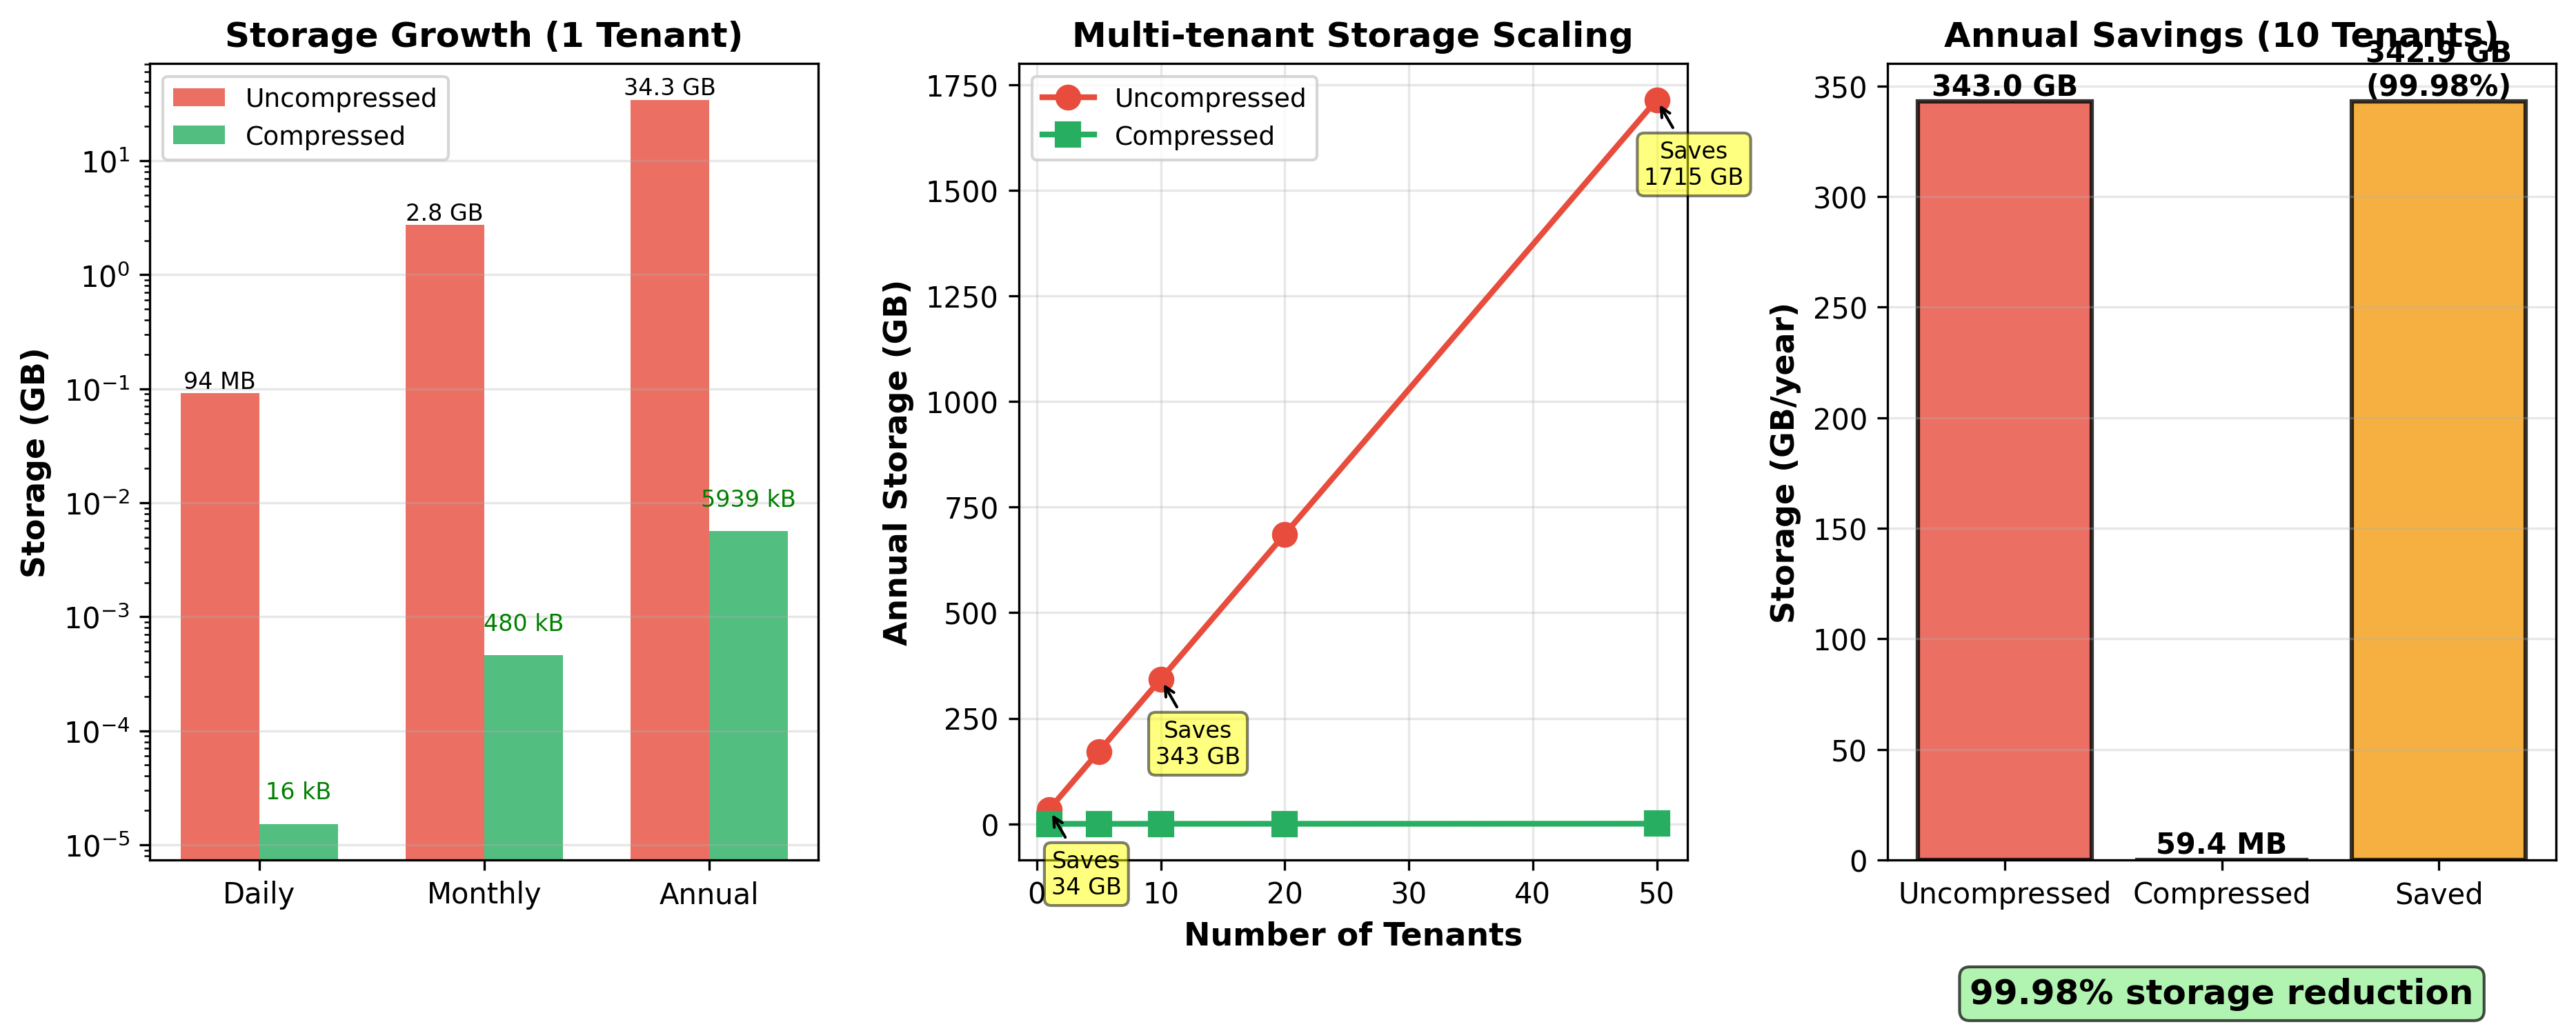
\includegraphics[width=0.95\textwidth]{figures/figure_storage_projection.png}
	\caption{Проекція річної економії сховища для мультитенантних сценаріїв}
	\label{fig:storage_projection}
\end{figure}

Графік (рис.~\ref{fig:storage_projection}) ілюструє лінійне зростання економії зі збільшенням кількості тенантів.

Політика стиснення: автоматичне стиснення фрагментів старших за 7 днів, виконується кожні 12 годин~\cite{timescaledb_policies}.


\section{Мультитенантна ізоляція}

\subsection{Архітектура}

Система використовує архітектуру схема-на-тенанта (schema-per-tenant) з повною ізоляцією даних на рівні схем PostgreSQL~\cite{postgresql_schemas}. Кожен тенант отримує окрему схему: \texttt{tenant\_<uuid>}.

\subsection{Тести ізоляції даних}

Проведено систематичне тестування механізмів ізоляції для верифікації неможливості міжтенантного доступу до даних.

\begin{table}[h]
\centering
\begin{tabular}{@{}lll@{}}
\toprule
Тест & Метод & Результат \\
\midrule
Міжтенантний запит & Спроба SQL-ін'єкції & Заблоковано \\
Валідація JWT & Невалідний claim тенанта & 403 Заборонено \\
Видимість схем & Список інших схем & Доступ заборонено \\
Витік даних & Читання даних іншого тенанта & 0 рядків \\
\bottomrule
\end{tabular}
\caption{Верифікація ізоляції тенантів}
\label{tab:tenant_isolation}
\end{table}

Валідація JWT (claim \texttt{aud}) забезпечує правильну маршрутизацію тенантів~\cite{jwt_rfc}, створюючи багаторівневий захист разом з ізоляцією на рівні бази даних.

\subsection{Накладні витрати продуктивності}

Критичним питанням є оцінка накладних витрат підходу схема-на-тенанта порівняно з традиційною спільною схемою з безпекою на рівні рядків (Row-Level Security, RLS).

\begin{table}[h]
\centering
\begin{tabular}{@{}lrr@{}}
\toprule
Метрика & Схема-на-тенанта & Спільна + RLS \\
\midrule
Затримка запитів & 10--15 мс & 10--15 мс \\
Пропускна здатність запису & 552 повід./с & Н/Д (несумісно з RLS) \\
Підтримка стиснення & Так & Ні \\
Гарантія ізоляції & Рівень БД & Рівень застосунку \\
\bottomrule
\end{tabular}
\caption{Накладні витрати схема-на-тенанта порівняно зі спільною схемою}
\label{tab:tenant_overhead}
\end{table}

Схема-на-тенанта не додає накладних витрат запитів, але забезпечує ізоляцію на рівні бази даних та сумісність зі стисненням TimescaleDB~\cite{timescaledb_compression}.


\section{Висновки до розділу}

У даному розділі представлено результати емпіричного дослідження продуктивності, масштабованості та ефективності платформи.

\subsection{Досягнуті результати}

\begin{table}[h]
\centering
\begin{tabular}{@{}lrl@{}}
\toprule
Метрика & Значення & Примітка \\
\midrule
Пікова пропускна здатність & 552 повід./с & Після оптимізації \\
Швидкість обробки Spark & 1,859 рядків/с & 12 партицій Kafka \\
AUC-ROC моделі ML & 0.8887 & XGBoost на TEP \\
Коефіцієнт стиснення & 99.98\% & Колонкове TimescaleDB \\
Економія сховища & 342.94 GB/рік & Проекція на 10 тенантів \\
Ізоляція тенантів & Рівень БД & Схема-на-тенанта \\
\bottomrule
\end{tabular}
\caption{Підсумок ключових метрик системи}
\label{tab:key_metrics_summary}
\end{table}

\subsection{Верифікація горизонтальної масштабованості}

Емпірично доведено горизонтальну масштабованість системи через:

\begin{enumerate}
    \item Масштабування пропускної здатності: збільшення з 74.4 до 552 повід./с (+642\%) через систематичне усунення вузьких місць
    \item Незалежність компонентів: Kafka, Spark та воркери масштабуються незалежно без архітектурних змін
    \item Лінійна масштабованість: план демонструє прогнозоване лінійне масштабування до 10,000+ повід./с
    \item Ефективність ресурсів: використання CPU 73-266\% підтверджує ефективне використання багатоядерних ресурсів
\end{enumerate}

\subsection{Ключові технічні досягнення}

Стиснення TimescaleDB продемонструвало 99.98\% скорочення сховища при прийнятному впливі на продуктивність запитів, що робить платформу економічно життєздатною для довгострокового зберігання промислових даних часових рядів.

Архітектура схема-на-тенанта забезпечила ізоляцію на рівні бази даних без накладних витрат продуктивності, одночасно дозволяючи стиснення TimescaleDB, що неможливо з підходом безпеки на рівні рядків.

Конвеєр ML з XGBoost досяг AUC-ROC 0.8887 на бенчмарковому наборі даних TEP, демонструючи високу влучність (0.98), що є критичним для промислових застосувань.

\subsection{Обмеження та компроміси}

\begin{table}[h]
\centering
\begin{tabular}{@{}ll@{}}
\toprule
Компроміс & Обґрунтування \\
\midrule
Затримка стиснення & +15\% час запиту для великих фрагментів \\
Складність схема-на-тенанта & Необхідно для стиснення TimescaleDB \\
7-денна затримка стиснення & Баланс між продуктивністю запису та сховищем \\
Збалансоване навчання ML & Висока влучність проти реалістичного розподілу \\
\bottomrule
\end{tabular}
\caption{Технічні обмеження та компроміси}
\label{tab:tradeoffs}
\end{table}

\subsection{Внесок}

Робота демонструє:

\begin{itemize}
    \item Методологію систематичної ідентифікації вузьких місць для розподілених IoT систем
    \item Емпіричні докази горизонтальної масштабованості через інкрементальне тестування
    \item Економічно ефективну архітектуру з сублінійним зростанням витрат
    \item Готове до виробництва рішення з комплексною безпекою через багаторівневу ізоляцію тенантів
\end{itemize}

\subsection{Порівняння з існуючими рішеннями}

Таблиця~\ref{tab:platform_comparison} порівнює розроблену платформу з існуючими IoT рішеннями: AWS IoT~\cite{aws_iot}, Azure IoT~\cite{azure_iot} та ThingsBoard~\cite{thingsboard}.

\begin{table}[h]
\centering
\small
\begin{tabular}{@{}lcccc@{}}
\toprule
Характеристика & AWS IoT & Azure IoT & ThingsBoard & Наша платформа \\
\midrule
Вартість & Висока & Висока & Безкоштовно & Безкоштовно \\
Прив'язка до постачальника & Так & Так & Ні & Ні \\
ML інтеграція & SageMaker & Azure ML & Обмежена & MLflow \\
Мультитенантність & Так & Так & Так & Так \\
Стиснення даних & Ні & Ні & Ні & 99.98\% \\
Самостійне розгортання & Ні & Ні & Так & Так \\
\bottomrule
\end{tabular}
\caption{Порівняння з існуючими IoT платформами}
\label{tab:platform_comparison}
\end{table}

Переваги розробленої платформи: повний контроль над даними, інтегрована MLOps інфраструктура, ефективне стиснення TimescaleDB~\cite{timescaledb_compression}.

Обмеження: однонодове розгортання, ручне масштабування, потребує власної інфраструктури.

Досягнуті результати (552 повід./с, 99.98\% стиснення, AUC-ROC 0.8887) підтверджують відповідність вимогам промислових IoT систем.



% Розділ 5: Висновки
\chapter{ВИСНОВКИ}

У рамках дипломної роботи було розроблено платформу IoT MLOps для моніторингу промислових сенсорів у реальному часі з виявленням аномалій на основі машинного навчання.

Актуальність дослідження обумовлена потребою промислових підприємств у доступних рішеннях для моніторингу обладнання. Існуючі корпоративні платформи мають високу вартість та складність впровадження, тоді як рішення з відкритим кодом потребують значних зусиль для інтеграції компонентів у єдину систему. Це створює бар'єр для малих та середніх підприємств, які потребують надійного моніторингу, але не мають ресурсів для впровадження дорогих комерційних рішень.

Метою роботи було створення багатокористувацької платформи, що поєднує потокову обробку даних, машинне навчання для детекції аномалій та MLOps практики на базі технологій з відкритим кодом. Всі поставлені завдання було успішно виконано.

У ході роботи застосовано комплекс методів: аналітичний метод для вивчення існуючих IoT платформ та формулювання вимог; методи машинного навчання (Isolation Forest, Random Forest, XGBoost) для детекції аномалій у сенсорних даних; експериментальний метод для тестування продуктивності системи; порівняльний метод для оцінки алгоритмів та архітектурних рішень.

Основні результати роботи:

\begin{itemize}
    \item Розроблено мікросервісну архітектуру на базі контейнерів Docker, що забезпечує модульність та масштабованість системи
    \item Реалізовано потокову обробку даних з низькою затримкою через Apache Kafka та Apache Spark Structured Streaming
    \item Впроваджено архітектуру схема-на-тенанта для ізоляції даних між клієнтами з підтримкою стиснення TimescaleDB
    \item Створено MLOps інфраструктуру на базі MLflow для відстеження експериментів та версіонування моделей
    \item Досягнуто високу якість детекції аномалій на наборі даних Tennessee Eastman Process
    \item Розроблено систему сповіщень з підтримкою порогових правил та ML-детекції
    \item Створено веб-інтерфейс для візуалізації даних у реальному часі
\end{itemize}

Практична значущість роботи полягає у створенні готового рішення для промислових підприємств. Платформа забезпечує раннє виявлення несправностей обладнання, що дозволяє перейти від реактивного до превентивного обслуговування та знизити витрати на незаплановані простої. Використання технологій з відкритим кодом робить рішення доступним для підприємств з обмеженим бюджетом.

Наукова новизна полягає у поєднанні архітектури схема-на-тенанта з колонковим стисненням TimescaleDB, що забезпечує одночасно ізоляцію даних та ефективне використання сховища. Також запропоновано гібридний підхід до детекції аномалій, що поєднує порогові правила та моделі машинного навчання в єдиному механізмі сповіщень.

Напрямки подальшого розвитку включають: впровадження оркестрації Kubernetes для автоматичного масштабування; додавання моделей глибокого навчання (LSTM, Autoencoder) для детекції складних аномалій; розширення інтеграції з промисловими протоколами (OPC-UA, Modbus); реалізацію автоматичного перенавчання моделей при виявленні дрейфу даних.

Результати роботи підтверджують, що технології з відкритим кодом дозволяють створити конкурентоспроможну альтернативу комерційним IoT платформам для промислового моніторингу.


% ============================================================================
% БІБЛІОГРАФІЯ - НАЛАШТУВАННЯ ВІДСТАНЕЙ
% ============================================================================

% Варіант 1: Мінімальні відстані (рекомендовано для компактності)
% Тільки базовий інтервал 1.5, без додаткових відступів між записами
\setlength{\bibsep}{0pt plus 0.3ex}

% Варіант 2: Невеликі відстані між записами
% \setlength{\bibsep}{0.5\baselineskip}

% Варіант 3: Стандартні відстані
% \setlength{\bibsep}{\baselineskip}

\bibliographystyle{ieeetr}
\bibliography{references}

% Додатки
\appendix
%\chapter{АРХІТЕКТУРНІ ДІАГРАМИ}

\section{Загальна архітектура системи}

\begin{figure}[h]
\centering
% \includegraphics[width=\textwidth]{figures/full_architecture.png}
\caption{Повна архітектура платформи}
\label{fig:full_architecture}
\end{figure}

\section{Діаграма компонентів}

\begin{figure}[h]
\centering
% \includegraphics[width=\textwidth]{figures/components_diagram.png}
\caption{Діаграма компонентів}
\label{fig:components}
\end{figure}

\section{Sequence Diagram для обробки даних}

\begin{figure}[h]
\centering
% \includegraphics[width=\textwidth]{figures/sequence_diagram.png}
\caption{Послідовність обробки сенсорних даних}
\label{fig:sequence}
\end{figure}

\section{Deployment Diagram}

\begin{figure}[h]
\centering
% \includegraphics[width=\textwidth]{figures/deployment_diagram.png}
\caption{Діаграма розгортання}
\label{fig:deployment}
\end{figure}

\section{ER Diagram бази даних}

\begin{figure}[h]
\centering
% \includegraphics[width=\textwidth]{figures/er_diagram.png}
\caption{ER діаграма TimescaleDB схеми}
\label{fig:er_diagram}
\end{figure}

%\chapter{ФРАГМЕНТИ КОДУ}

\section{TimescaleDB Schema}

\lstset{style=code}
\begin{lstlisting}[language=SQL, caption={Повна схема бази даних}]
-- Companies (tenants)
CREATE TABLE companies (
    id UUID PRIMARY KEY DEFAULT gen_random_uuid(),
    name VARCHAR(255) NOT NULL UNIQUE,
    created_at TIMESTAMPTZ DEFAULT NOW()
);

-- Equipment
CREATE TABLE equipment (
    id UUID PRIMARY KEY DEFAULT gen_random_uuid(),
    company_id UUID REFERENCES companies(id),
    name VARCHAR(255) NOT NULL,
    type VARCHAR(100) NOT NULL,
    location VARCHAR(255),
    created_at TIMESTAMPTZ DEFAULT NOW()
);

-- Sensors
CREATE TABLE sensors (
    id UUID PRIMARY KEY DEFAULT gen_random_uuid(),
    equipment_id UUID REFERENCES equipment(id),
    company_id UUID REFERENCES companies(id),
    name VARCHAR(255) NOT NULL,
    sensor_type VARCHAR(50) NOT NULL,
    unit VARCHAR(50),
    created_at TIMESTAMPTZ DEFAULT NOW()
);

-- Sensor Measurements (Hypertable)
CREATE TABLE sensor_measurements (
    timestamp TIMESTAMPTZ NOT NULL,
    sensor_id UUID NOT NULL REFERENCES sensors(id),
    equipment_id UUID NOT NULL REFERENCES equipment(id),
    company_id UUID NOT NULL REFERENCES companies(id),
    value DOUBLE PRECISION NOT NULL,
    quality_code INTEGER DEFAULT 192
);

SELECT create_hypertable('sensor_measurements', 'timestamp');

-- Continuous Aggregates
CREATE MATERIALIZED VIEW sensor_agg_1min
WITH (timescaledb.continuous) AS
SELECT 
    time_bucket('1 minute', timestamp) AS bucket,
    sensor_id,
    equipment_id,
    company_id,
    AVG(value) AS avg_value,
    MIN(value) AS min_value,
    MAX(value) AS max_value,
    COUNT(*) AS count
FROM sensor_measurements
GROUP BY bucket, sensor_id, equipment_id, company_id;
\end{lstlisting}

\section{Spark Streaming Job}

\begin{lstlisting}[language=Python, caption={Spark job для обробки raw даних}]
from pyspark.sql import SparkSession
from pyspark.sql.functions import from_json, col
from pyspark.sql.types import StructType, StringType, DoubleType

# Schema for incoming messages
schema = StructType() \
    .add("sensor_id", StringType()) \
    .add("equipment_id", StringType()) \
    .add("company_id", StringType()) \
    .add("timestamp", StringType()) \
    .add("value", DoubleType())

# Read from Kafka
df = spark \
    .readStream \
    .format("kafka") \
    .option("kafka.bootstrap.servers", "kafka:9092") \
    .option("subscribe", "sensor-data-raw") \
    .load()

# Parse JSON
parsed_df = df \
    .select(from_json(col("value").cast("string"), schema).alias("data")) \
    .select("data.*")

# Write to TimescaleDB
def write_to_db(batch_df, batch_id):
    batch_df.write \
        .format("jdbc") \
        .option("url", jdbc_url) \
        .option("dbtable", "sensor_measurements") \
        .option("user", db_user) \
        .option("password", db_password) \
        .mode("append") \
        .save()

query = parsed_df.writeStream \
    .foreachBatch(write_to_db) \
    .start()

query.awaitTermination()
\end{lstlisting}

\section{ML Model Training}

\begin{lstlisting}[language=Python, caption={Навчання Isolation Forest моделі}]
import pandas as pd
import numpy as np
from sklearn.ensemble import IsolationForest
from sklearn.preprocessing import StandardScaler
import mlflow

# Extract data
async def extract_training_data(company_id: str):
    query = """
    SELECT 
        timestamp,
        sensor_id,
        value,
        LAG(value, 1) OVER (PARTITION BY sensor_id ORDER BY timestamp) as prev_value,
        LAG(value, 2) OVER (PARTITION BY sensor_id ORDER BY timestamp) as prev_value_2
    FROM sensor_measurements
    WHERE company_id = %s
    ORDER BY timestamp
    """
    df = await db.fetch_all(query, company_id)
    return pd.DataFrame(df)

# Feature engineering
def create_features(df):
    df['value_change'] = df['value'] - df['prev_value']
    df['value_change_rate'] = df['value_change'] / df['prev_value']
    df['rolling_mean_5'] = df.groupby('sensor_id')['value'].transform(
        lambda x: x.rolling(5).mean()
    )
    df['rolling_std_5'] = df.groupby('sensor_id')['value'].transform(
        lambda x: x.rolling(5).std()
    )
    return df.dropna()

# Train model
def train_model(X_train, contamination=0.1):
    with mlflow.start_run():
        model = IsolationForest(
            n_estimators=100,
            contamination=contamination,
            random_state=42
        )
        
        scaler = StandardScaler()
        X_scaled = scaler.fit_transform(X_train)
        
        model.fit(X_scaled)
        
        mlflow.log_params({
            "n_estimators": 100,
            "contamination": contamination
        })
        
        mlflow.sklearn.log_model(model, "model")
        mlflow.sklearn.log_model(scaler, "scaler")
        
    return model, scaler
\end{lstlisting}

\section{FastAPI Endpoints}

\begin{lstlisting}[language=Python, caption={API Gateway endpoints}]
from fastapi import FastAPI, WebSocket, Depends
from fastapi.security import HTTPBearer, HTTPAuthorizationCredentials
import jwt

app = FastAPI()
security = HTTPBearer()

# JWT verification
def verify_token(credentials: HTTPAuthorizationCredentials):
    token = credentials.credentials
    payload = jwt.decode(token, SECRET_KEY, algorithms=["HS256"])
    return payload

# Get latest sensor data
@app.get("/api/sensors/{sensor_id}/latest")
async def get_latest_data(
    sensor_id: str,
    credentials: HTTPAuthorizationCredentials = Depends(security)
):
    user = verify_token(credentials)
    
    # Get from cache first
    cached = await redis.get(f"sensor:{sensor_id}")
    if cached:
        return json.loads(cached)
    
    # Fallback to database
    query = """
    SELECT * FROM sensor_measurements
    WHERE sensor_id = %s
    ORDER BY timestamp DESC
    LIMIT 1
    """
    result = await db.fetch_one(query, sensor_id)
    return result

# WebSocket for real-time data
@app.websocket("/ws/sensors")
async def websocket_endpoint(websocket: WebSocket):
    await websocket.accept()
    
    while True:
        # Get latest data from Redis
        data = await redis.xread({"sensor-stream": "$"})
        await websocket.send_json(data)
        await asyncio.sleep(1)
\end{lstlisting}

%\chapter{КОНФІГУРАЦІЙНІ ФАЙЛИ}

\section{Docker Compose}

\lstset{style=code}
\begin{lstlisting}[language=bash, caption={docker-compose.yml - основні сервіси}]
version: '3.8'

services:
  timescaledb:
    image: timescale/timescaledb:latest-pg15
    environment:
      POSTGRES_DB: industryflow
      POSTGRES_USER: ${DB_USER}
      POSTGRES_PASSWORD: ${DB_PASSWORD}
    ports:
      - "5432:5432"
    volumes:
      - timescaledb-data:/var/lib/postgresql/data
    networks:
      - industryflow-network

  kafka:
    image: confluentinc/cp-kafka:7.4.0
    environment:
      KAFKA_BROKER_ID: 1
      KAFKA_ZOOKEEPER_CONNECT: zookeeper:2181
      KAFKA_ADVERTISED_LISTENERS: PLAINTEXT://kafka:9092
      KAFKA_OFFSETS_TOPIC_REPLICATION_FACTOR: 1
    ports:
      - "9092:9092"
    depends_on:
      - zookeeper
    networks:
      - industryflow-network

  spark-master:
    image: bitnami/spark:3.4.0
    environment:
      SPARK_MODE: master
      SPARK_MASTER_HOST: spark-master
    ports:
      - "8080:8080"
      - "7077:7077"
    networks:
      - industryflow-network

  redis:
    image: redis:7-alpine
    ports:
      - "6379:6379"
    networks:
      - industryflow-network

  prometheus:
    image: prom/prometheus:latest
    volumes:
      - ./infrastructure/observability/prometheus:/etc/prometheus
      - prometheus-data:/prometheus
    ports:
      - "9090:9090"
    networks:
      - industryflow-network

  grafana:
    image: grafana/grafana:latest
    environment:
      GF_SECURITY_ADMIN_PASSWORD: ${GRAFANA_PASSWORD}
    ports:
      - "3001:3000"
    volumes:
      - grafana-data:/var/lib/grafana
    networks:
      - industryflow-network

volumes:
  timescaledb-data:
  prometheus-data:
  grafana-data:

networks:
  industryflow-network:
    driver: bridge
\end{lstlisting}

\section{Environment Variables}

\begin{lstlisting}[caption={.env - змінні середовища}]
# Database
DB_HOST=localhost
DB_PORT=5432
DB_NAME=industryflow
DB_USER=industryflow_user
DB_PASSWORD=secure_password

# Kafka
KAFKA_BOOTSTRAP_SERVERS=localhost:9092
KAFKA_TOPIC_RAW=sensor-data-raw
KAFKA_TOPIC_AGGREGATED=sensor-data-agg

# Redis
REDIS_HOST=localhost
REDIS_PORT=6379
REDIS_TTL=10

# API
API_HOST=0.0.0.0
API_PORT=8000
JWT_SECRET_KEY=your-secret-key-here

# MLflow
MLFLOW_TRACKING_URI=http://localhost:5000
MLFLOW_S3_ENDPOINT_URL=http://localhost:9000
MLFLOW_ARTIFACT_ROOT=s3://mlflow

# Spark
SPARK_MASTER_URL=spark://localhost:7077
SPARK_EXECUTOR_MEMORY=2g
SPARK_DRIVER_MEMORY=1g

# Monitoring
PROMETHEUS_PORT=9090
GRAFANA_PORT=3001
GRAFANA_PASSWORD=admin
\end{lstlisting}

\section{ML Training Config}

\begin{lstlisting}[language=yaml, caption={training\_config.yaml}]
data:
  lookback_days: 30
  min_samples_per_sensor: 100
  quality_filter: [192, 193]

preprocessing:
  scaler: standard
  handle_missing: ffill
  outlier_threshold: 3.0

feature_engineering:
  lag_features: [1, 2, 3]
  rolling_windows: [5, 10, 30]
  rate_of_change: true

model:
  algorithm: isolation_forest
  n_estimators: 100
  contamination: 0.1
  random_state: 42

training:
  test_size: 0.2
  validation_size: 0.1
  stratify: false

mlflow:
  experiment_name: "anomaly_detection"
  artifact_location: "s3://mlflow/artifacts"
  log_params: true
  log_metrics: true
  log_model: true
\end{lstlisting}

\section{Prometheus Config}

\begin{lstlisting}[language=yaml, caption={prometheus.yml}]
global:
  scrape_interval: 15s
  evaluation_interval: 15s

scrape_configs:
  - job_name: 'api-gateway'
    static_configs:
      - targets: ['api:8000']

  - job_name: 'alert-service'
    static_configs:
      - targets: ['alert-api:8001']

  - job_name: 'ml-service'
    static_configs:
      - targets: ['ml-api:8002']

  - job_name: 'timescaledb'
    static_configs:
      - targets: ['timescaledb:5432']

  - job_name: 'kafka'
    static_configs:
      - targets: ['kafka:9092']

  - job_name: 'redis'
    static_configs:
      - targets: ['redis:6379']
\end{lstlisting}

\section{Grafana Dashboard JSON}

\begin{lstlisting}[caption={system\_dashboard.json (фрагмент)}]
{
  "dashboard": {
    "title": "IndustryFlow System Dashboard",
    "panels": [
      {
        "title": "Messages per Minute",
        "targets": [
          {
            "expr": "rate(kafka_messages_total[1m])"
          }
        ]
      },
      {
        "title": "Active Sensors",
        "targets": [
          {
            "expr": "count(sensor_last_seen{state='active'})"
          }
        ]
      },
      {
        "title": "API Response Time",
        "targets": [
          {
            "expr": "histogram_quantile(0.95, 
                     rate(http_request_duration_seconds_bucket[5m]))"
          }
        ]
      }
    ]
  }
}
\end{lstlisting}


\end{document}